%% Dokumenteinstellungen
\documentclass[12pt,german]{report}

%% Verwendete Pakete
\usepackage[T1]{fontenc}
\usepackage[latin1]{inputenc}
\usepackage{times}
\usepackage{geometry}
\geometry{verbose,a4paper,tmargin=4cm,bmargin=4cm,lmargin=2.8cm,rmargin=2.8cm}
\usepackage{babel}
\usepackage{graphicx}
\usepackage{titlesec}
\usepackage{setspace}
\usepackage{listings}
\titleformat{\chapter}{\huge}{\thechapter.}{20pt}{\huge}

%% Einstellungen
\setlength{\oddsidemargin}{0cm}
\setlength{\topmargin}{-1.5cm}
\setlength{\textheight}{22cm}
\setlength{\textwidth}{16cm}
\setlength{\headsep}{1cm}
\setlength{\parindent}{0ex}
\setlength{\parskip}{2.0ex plus 0.9ex minus 0.4ex}

\begin{document}

%% Titelblatt
\input{ba_titel.tex}
\newpage 
\thispagestyle{empty}
\quad 
\newpage

%% Inhaltsverzeichnis
\tableofcontents
\newpage 
\thispagestyle{empty}
\quad 
\newpage

%% Formaljuristisches
%%
%% Formaljuristisches
%%
\chapter*{Best\"atigung}

Hiermit versichere ich, dass die vorliegende Arbeit selbst\"andig verfasst und keine anderen als die angegebenen Quellen und Hilfsmittel benutzt wurden.

Ferner habe ich vom Merkblatt \"uber die Verwendung von Abschlussarbeiten Kenntnis genommen und r\"aume das einfache Nutzungsrecht an meiner Arbeit der Universit\"at der Bundeswehr M\"unchen ein.

\vspace{1cm}

Neubiberg, den 10.09.2020

\vspace{2cm} 

Lina Suttrup

\newpage 
\thispagestyle{empty}
\quad 
\newpage

%% Einzeldokumente, z.B. in Kapitel aufgeteilt

\begin{onehalfspace}
%%
%% Kapitel
%%
\chapter{Einleitung}
Was w\"are, wenn Computer von ihren Erfahrungen lernen k\"onnten, so wie Menschen es tun? Eine Frage, aus der viele Forschungsfelder entsprungen sind. \textbf{K\"unstliche Intelligenz} ist ein gro{\ss}es Themengebiet, aber ohne \textbf{Machine Learning} sind Computer nicht "`schlauer"' als die Programme, die sie ausf\"uhren - und die von Menschen programmiert werden. Zwar kann ein Computer ein Problem mit vorgegebenen L\"osungsweg meist weit schneller l\"osen als der Mensch selber, aber wie kommt er auf diesen L\"osungsweg? \textbf{Machine Learning} und\textbf{ Deep Learning} konzentrieren sich auf genau diese Problemstellung.\\
Seit der Entwicklung erster \textbf{Machine Learning} Algorithmen hat dieses Feld immense Fortschritte gemacht, besonders in den letzten Jahren, in denen auch \textbf{Deep Learning} durch die Entwicklung immer schnellerer Prozessoren sowie der M\"oglichkeiten der modernen GPUs zur Parallelisierung von Aufgaben immer weiter in den Vordergrund r\"ucken konnte.
Machine Learning und \textbf{Deep Learning} ist heute schon weit verbreitet und wird in den verschiedensten Feldern eingesetzt - von  E-Mail Spam Klassifizierung bis hin zur Erkennung von Tumoren auf R\"ontgenbildern, es bleibt aber weiterhin ein gro{\ss}es Forschungsfeld.


\section{Natural Language Processing}
%Quellen
Ein wichtiger Teil der K\"unstlichen Intelligenz ist die \textbf{Computerlinguistik}, oder auch \textbf{Natural Language Processing (NLP)}. Menschliche Sprache ist f\"ur Maschinen nur schwer verst\"andlich, da sie im Gegensatz zu Maschinensprachen keiner genauen Logik folgen: Sie ist im Grunde unvorhersehbar und f\"uhrt selbst bei Menschen zu Missverst\"andnissen. Trotzdem gibt es heutzutage viele Anwendungen von \textbf{NLP} im Alltag, und Beispiele wie die heutigen Sprachassistenten zeigen, wie weit dieses Feld in einer sehr kurzen Zeit voranschreiten konnte.\\
Aufgrund der Komplexit\"at des Problems gibt es meherer Herangehensweisen, um nat\"urliche Sprache f\"ur Maschinen verst\"andlich zu machen. Ihnen allen ist gemein, dass sie Sprache durch Zahlen repr\"asentieren. \\
Es gibt Ans\"atze, die W\"orter als einzelne Einheiten nehmen, und diesen einfach eine Zahl zuordnen. Dies hat den Vorteil, dass es leicht umzusetzen ist und auch keine hohe Anzahl an Trainingsdaten braucht. Das Problem daran ist, dass so sehr viel Bedeutung verloren gehen kann - in nat\"urlicher Sprache sind h\"aufig die umgebenden W\"orter genauso wichtig wie das betrachtete Wort. Kontext und Wortzusammenh\"ange gehen durch diesen Ansatz verloren.\\
Eine weitere bekannte Technik ist der Einsatz von \textbf{Wortverktoren}, die durch ihre hohe Dimensionalit\"at viele Beziehungen zwischen W\"ortern bewahren k\"onnen. Diese Repr\"asentation ist vielversprechend, aber auch hier kann nicht immer der Kontext gewahrt werden, da einem Wort genau ein Vektor zugeordnet wird.\\
Eine Verbesserung, nicht nur in diesem Aspekt, bringen \textbf{Sprachmodelle}. Sie k\"onnen vielf\"altig eingesetzt werden, haben einen gro{\ss}en Wortschatz in verschiedenen Sprachen und sind vortrainiert - sie m\"ussen entsprechend nur der Aufgabe angepasst werden, was einer enormen Zeitersparnis entspricht. Durch Feinabstimmung der verschiedenen Parameter kann bei Sprachmodellen auch viel erreicht werden \cite{imagenet_moment}.

\section{Sentiment Analysis}
\textbf{Sentiment Analysis} ist die Einordnung von Text in Kategorien von Emotionen, wobei es verschiedene Skalen gibt. Die einfachste ist hierbei die Einordnung in "`Neutral"', "`Positiv"' und "`Negativ"', aber es gibt auch Zuordnungen zu Werten von -1 bis 1 oder anderen Zahlenwerten. Diese Werte werden nicht immer mit einheitlicher Bedeutung genutzt. 


\section{Stance detection}
Bei \textbf{Stance Detection} geht es darum, herauszufinden, wie die Haltung des Autors eines Textes zu einer bestimmten These oder einem allgemeinen Begriff ist. Beste Ergebnisse wurden durch Unterteilung der Aufgabe in zwei Schritte erzielt; Zun\"achst wird \textbf{Topic Modeling} genutzt, um herauszufinden, ob der Text \"uberhaupt mit der Stance in Verbindung gebracht werden kann. Daraufhin wird, falls dies der Fall ist, auf die Stance bezogene \textbf{Sentiment Analysis} genutzt, um die Haltung des Autors zu ermitteln.


\section{Zielsetzung und Vorgehen}
Ziel dieser Arbeit ist es, zu erforschen wie gut sich verschiedene \textbf{Sprachmodelle} zum Einsatz in \textbf{Sentiment Analysis} und \textbf{Stance Detection} eignen.
Dazu werden die verschiedenen Modelle vorgestellt und analysiert, welche f\"ur den Einsatz in Frage kommen, da die Modelle durch unterschiedlichen Aufbau oder auch verf\"ugbare Datens\"atze nicht alle gleich gute Herangehensweisen an die Problemstellung darstellen.
F\"ur die Versuche werden mehrere \textbf{Corpora} verwendet, von denen die meisten \"offentlich zug\"anglich sind. Die  \textbf{Corpora} bestehen aus Tweets, die sich aufgrund der limitierten Zeichenl\"ange und der Popularit\"at  der Plattform \textit{Twitter} gut f\"ur die Auswertung in beiden Aufgaben eignen oder aus Artikeln, die f\"ur \textbf{Stance detection} eine gute Grundlage bieten.
Die Ergebnisse werden ausgewertet und miteinander verglichen.





%%
%% Kapitel
%%
\chapter{Sprachmodelle}
Bis zur Einf\"uhrung von Sprachmodellen gab es f\"ur NLP in Machine Learning ein gro{\ss}es Problem: Textdaten, wie auch Sprache, sind inherent sequentiell. Im Gegensatz zu Bildern, bei denen alle Daten auf einmal verarbeitet werden k\"onnen, konnte die Textverarbeitung die Beschleunigung durch den Einsatz von GPUs nicht nutzen, da viele Aufgaben nicht parallelisiert werden konnten \cite{attention}.\\ Weiterhin gab es keine M\"oglichkeit, ein schon vortrainiertes Modell f\"ur andere Aufgaben weiter zu verwenden, da das Training f\"ur die verschiedenen Aufgaben und auch Dom\"anen sehr spezifisch angegangen werden muss. Diese Faktoren f\"uhrten zu einem deutlichen Mehraufwand von NLP z.B. gegen\"uber Bildverarbeitung.\\
Das Ziel von Sprachmodellen ist es, parallele Verarbeitung der Daten m\"oglich zu machen sowie, im Gegensatz zu vortrainierten \textbf{Wortvektor Embeddings} wie \textbf{GLoVe} den Kontext der einzelnen W\"orter im Satz zu wahren. In den Embeddings wird jedem Wort ein Vektor zugewiesen, sodass \"ahnliche W\"orter nah beieinander liegen und die Beziehung zwischen W\"ortern erhalten bleibt. Dadurch k\"onnen interessante Rechnungen aufgestellt werden:
\begin{verbatim} 
London - England + Spanien = Madrid
\end{verbatim} 
Mit ganzen Textsequenzen k\"onnen aber auch diese Vektor Embeddings aufgrund der fehlenden Kontextinformationen nur bedingt gut umgehen.



\section{Problemstellung}
Wie schon erw\"ahnt muss Sprache sequentiell versarbeitet werden. Dazu werden meist \textbf{Gated RNNs} und \textbf{Long Short Term Memory (LSTM)} - Netzwerke verwendet \cite{attention}. Durch einige Techniken kann man mit diesen Netzen auch gute Laufzeiten erreichen, aber es besteht ein weiteres Problem: Der Kontext der W\"orter geht schnell verloren, da diese Netze einem Wort meist auch nur eine Bedeutung zuordnen k\"onnen.Der Umstand, dass diese Netze f\"ur jede Anwendung spezifisch trainiert werden m\"ussen, macht ihren Einsatz sehr umst\"andlich.\\
Ein ebenfalls sehr gro{\ss}es Problem in NLP ist die Tatsache, dass \textbf{\"Uberwachtes Lernen} mit erheblichem manuellen Aufwand - dem Annotieren und Labeln der Daten - verbunden ist. Es gibt zwar sehr gro{\ss}e Mengen an Daten, die durch das Internet verf\"ugbar sind (z.B. alle \textit{Wikipedia-Artikel}, diese eignen sich aber nur f\"ur un\"uberwachte Lernmethoden, da sie nicht gelabelt sind. Die Menge an gelabelten Daten hingegen ist verschwinden gering im Vergleich zu allen frei verf\"ugbaren. Dies legt die Entwicklung eines Systems nahe, das mit \textbf{teil-} oder \textbf{fern\"uberwachtem Lernen} auskommt. Heutige Sprachmodelle versuchen hier anzusetzen, indem sie in einem ersten Schritt un\"uberwacht mit Korpussen unterschiedlicher Gr\"o{\ss}e die Repr\"asentation einer Sprache lernen, um dann im zweiten Schritt an die zu erf\"ullende Aufgabe angepasst zu werden. Besonders interessant hierbei sind neueste Entwicklungen \cite{gpt3}, durch die ein Modell sogar mit nur einem Beispiel der zu erf\"ullenden Aufgabe gute Ergebnisse erzielen kann. Dieses Konzept nennt sich \textbf{Transfer Learning}, durch Anwendung in der Bildverarbeitung konnten dadurch gro{\ss}e Verbesserungen in Zeit und Genauigkeit erreicht werden \cite{ulm}, da ein vortrainiertes Modell nur noch mit Feinabstimmungen f\"ur die sp\"atere Aufgabe vorbereitet werden muss.\\
Das grunds\"atzliche Ziel von Sprachmodellen ist die Ausgabe des Wortes, das am wahrscheinlichsten auf eine Eingabesequenz folgt. Direkt anwendbar ist dies z.B. auf Textgeneration und \"Ubersetzungen, w\"ahrend f\"ur andere Aufgaben leichte \"Anderungen vorgenommen werden m\"ussen um z.B. f\"ur \textbf{Sentiment Analysis} eine Zahl zu erhalten, die dem in der Eingabe erkannten Sentiment entspricht. Sieht man diese Zahl als das vorrauszusagende Wort an k\"onnen diese \"Anderungen recht leicht umgesetzt werden.



\section{Sprachmodelle auf Basis von LSTMs}
\textbf{LSTMs} k\"onnen aufgrund ihrer Architektur gut mit kurzen S\"atzen umgehen, aber je l\"anger die Wortsequenz, desto schlechter kann sie verarbeitet werden: Es gibt dabei Probleme mit \textbf{vanishing} oder \textbf{exploding gradients}, je nach Einstellung der Parameter.\\
Durch die sequentiellen Verarbeitung steigt die Verarbeitungszeit mit der Textl\"ange an, wodurch \textbf{LSTMs} generell langsamer sind als \textbf{RNNs}, da die Neuronen komplexer sind.\\
Trotz dieser Nachteile k\"onnen mit dieser Architektur f\"ur einige Anwendungen geeignete Sprachmodelle erstellt werden.


\subsection{ELMo}
\textbf{ELMo} baut auf der Idee der Wortvektoren oder auch \textbf{Word Embeddings} auf. Die von \textbf{ELMo} erlernten Wort-Embeddings k\"onnen in den eigenen, f\"ur Aufgaben spezifisch entwickelten Netzen eingebunden werden, um gegen\"uber sehr festgelegter Vektoren wir \textbf{GloVe} Ergenisse zu erzielen, die zum Zeitpunkt der Entwicklung dieses Modells zu den besten geh\"orten \cite{elmo}.\\

\textbf{Architektur}\\
\begin{figure}[!ht]
\centering
\includegraphics[height=5cm]{pics/elmo_layered_embeddings.png}
\caption{Aufbau des ELMo-Modells \cite{elmoex}}
\label{fig:elmo_layers}
\end{figure}
Die zweischichtige Architektur besteht aus jeweils einem \textbf{Feed-Forward} Netz, dessen Layer in Abbildung \ref{fig:elmo_layers} in rot eingezeichnet sind und einem \textbf{Feed-Backward} Netz, das in blau dargestellt ist. Damit ist \textbf{ELMo} ein sogenanntes \textbf{bidirektionales Sprachmodell}. Die Schichten bestehen aus jeweils 4096 LSTM-Zellen und zwischen den zwei Schichten gibt es eine Verbindung zur Eingabeschicht.\\

\textbf{Input und Output}\\
Wie in der Abbildung \ref{fig:elmo_layers} zu sehen, gibt es drei Repr\"asentationen f\"ur ein Wort, eine in jeder Schicht. Zusammengenommen ergeben sie das ELMo Embedding.
\begin{figure}[!ht]
\centering
\includegraphics[height=5cm]{pics/elmo_character_token.png}
\caption{Vorverarbeitung der W\"orter \cite{elmoex}}
\label{fig:elmo_character}
\end{figure}
Das erste Embedding der W\"orter entsteht schon vor dem eigentlichen Sprachmodell, wie Abbildung \ref{fig:elmo_character} zeigt. Die W\"orter werden in Character-Tokens aufgeteilt und in einem Convolutional Network mit 2048 Filtern und Max Pooling, gefolgt von einem zweischichtigen \textbf{Highway Netz} verarbeitet, bevor sie in das LSTM-Netz gegeben werden.\\

\textbf{Trainingdaten}\\
Das Modell wurde mit dem 1B Word Benchmark trainiert, dass einen Korpus von 0,8 Milliarden W\"ortern besteht und ist damit ein insgesamt sehr gro{\ss}es Modell.


\subsection{ULMFit}
\textbf{Universal Language Mdoel Fine-Tuning} oder auch \textbf{ULMFit} ist ein Vorschlag eines von der Architektur recht einfach gehaltenen Sprachmodells, das Transfer Learning in NLP zug\"anglich machen wollte. Der Ansatz ist besonders darauf fokussiert, ein mit allgemeinen Daten trainiertes Modell auf eine spezifische Aufgabe mit einem eigenen Kontext (z.B. Medizin, IT etc.) fein abzustimmen \cite{ulm}. Dadurch wird die Gr\"o{\ss}e des gelabelten Datensatzes und die Anzahl der dom\"anenspezifischen Dokumente, die f\"ur ein von Grund auf neu implementiertes Modell ben\"otigt w\"urden stark gemindert.\\

\textbf{Architektur}\\
Das Modell besteht aus drei LSTM-Schichten, die, um Overfitting auf den Daten zu vermeiden, mit einer sehr hohen Dropout-Rate versehen sind. Pro Schicht hat \textbf{ULMFit} 1150 versteckte Neuronen.\\
Bei der Arbeit mit \textbf{ULMFit} werden generell drei Schritte ausgef\"uhrt \cite{ulm}:
\begin{enumerate}
\item Trainieren des Modells mit einem allgemeinen, gro{\ss}en Datensatz 
\item Feinabstimmung des Sprachmodells f\"ur die NLP-Aufgabe
\item Feinabstimmung des Klassifikators f\"ur die Aufgabe
\end{enumerate}
Schritt 1. muss bei Einsatz des Modells nicht ausgef\"uhrt werden, da diese Version des Modells verf\"ugbar ist. Durch diesen Schritt lernt das Modell, in den verschiedenen Schichten die Merkmale der (in diesem Fall englischen) Sprache abzubilden. Bei Schritt 2. wird mit \textbf{discriminative Fine-Tuning} und einer abgeschr\"agten, dreieckigen Lernrate gearbeitet, um Merkmale der in der Aufgabe genutzen Sprache zu lernen. Diese Lernrate wird angewandt, da die verschiedenen Schichten unterschiedliche Merkmale lernen sollen und sich damit die letzten Schichten nicht mehr viel ver\"andern. Schritt 3. nutzt \textbf{gradual unfreezing} sowie die beiden in Schritt 2. genutzten Techniken f\"ur die Feinabstimmung. Hierf\"ur werden an das Sprachmodell zwei lineare Schichten mit ReLu Activation, dropout und Batchnormalisierung und eine Softmax-Schicht f\"ur die Ausgabe.\\

\textbf{Input und Output}\\
Die Input-Sequenzen werden vor der Verarbeitung in den LSTM-Schichten in 400 dimensionale Word Embeddings umgewandelt.\\
Wie bei Sprachmodellen \"ublich ist der Output von \textbf{ULMFit} eine Wahrscheinlichkeitsverteilung \"uber das Vokabular, um das mit h\"ochster Wahrscheinlichkeit als n\"achtes im Satz kommendes Wort auszugeben.\\

\textbf{Trainingsdaten}\\
\textbf{ULMFit} wurde mit dem Datensatz \textbf{Wikitext-103}, der aus 103 Millionen W\"ortern in Wikipedia Artikeln besteht. Die Feinabstimmung liefert schon mit 100 Datens\"atzen gute Ergebnisse \cite{ulm}.



\section{Sprachmodelle auf Basis von Transformern}
\textbf{Transformer} sind die Basis der heute meistgenutzten Sprachmodelle \cite{bert}\cite{gpt}. Sie wurden 2017 entwickelt, um das Problem der sequentiellen Verarbeitung in Maschineller \"Ubersetzung zu l\"osen: Als Eingabe kann ein \textbf{Transformer} eine ganze Textsequenz verarbeiten. Die wichtigste Komponente in diesem System ist \textbf{Attention}: Dadurch kann einem Wort sein Kontext innerhalb der betrachteten Sequenz zugeordnet werden.\\
\begin{figure}[!ht]
\centering
\includegraphics{pics/attention.jpg}
\caption{Aufbau eines Transformers \cite{attention}}
\label{fig:attention}
\end{figure}

\subsection*{Encoder}
Wie in Abbildung \ref{fig:attention} zu sehen, wird die Eingabe zun\"achst in Wortvektoren f\"ur jedes Eingabewort umgewandelt, die sich aus der Addition des Vektors im \textbf{Embedding Space} mit einem \textbf{Positionsvektor (Positional Encoding)}, der die Position des Wortes im Satz enth\"alt, ergibt. Der Positionsvektor wird durch Sinus- und Kosinusfunktionen bestimmt und ist wichtig, da Sequenzen parallel verarbeitet werden und die Position dadurch verloren geht. Dieser Eingabevektor wird an einen \textbf{Encoder} weitergegeben, der eine \textbf{Attention-Matrix} f\"ur die Eingabesequenz erstellt. Sie besteht aus einem Vektor der L\"ange der Textsequenz f\"ur jedes Wort. Diese Matrix enth\"alt Informationen dar\"uber, wie relevant die einzelnen W\"orter der Sequenz f\"ureinander sind: In dem Satz
\begin{verbatim} 
Der braune Hund
\end{verbatim} 
bezieht sich z.B. das Wort "`Der"' sowie das Adjektiv "`braune"' auf das Wort "`Hund"'. In dem Attention-Vektor w\"aren entsprechend die Werte f\"ur "`Hund"' in den Vektoren der beiden anderen W\"orter h\"oher. \textbf{Attention} ist der Schl\"usselpunkt f\"ur die Funktion der Transformer: Dadurch erhalten die Wortvektoren ihre eigentliche Kontextinformation. Um die Werte zu optimieren werden hier die Mittelwerte von acht Vektoren pro Wort ermittelt.\\
Alle bisher errechneten Vektoren werden danach aufaddiert, normalisiert und jeder Vektor wird in ein Feed-Forward-Netz gegeben. Hierbei kann parallelisiert werden, da die einzelnen Vektoren voneinander unabh\"angig sind. Die Ausgabe des \textbf{Encoders} sind die mit Kontext und Attention encodierten Wortvektoren.\\

\subsection*{Decoder}
Der \textbf{Decoder} ist \"ahnlich aufgebaut. Er nimmt einen zweiten Input an - der eigentliche Output bei Supervised Learning - der, wie Abbildung \ref{fig:attention} zeigt, zun\"achst auch in einen Eingabevektor mit Positionsinformation und Attention-Matrix umgewandelt wird. Im n\"achsten Schritt werden Input und Output gemeinsam in ein weiteres Netz zur Attention-Bestimmung gegeben, in dem die Attention Matrix der beiden Vektoren zueinander bestimmt wird: Die Frage die hierbei beantwortet wird ist, wie welche W\"orter in den beiden Sequenzen zueinander stehen. Dies ist gut an dem Beispiel der Sprach\"ubersetzung zu sehen, bei der der zu lernende Output der Input in einer anderen Sprache ist.
\begin{verbatim} 
The brown dog
\end{verbatim} 
w\"are entsprechend hier der Output (Decoder Input). Es wird in diesem Schritt analysiert, wie das Wort "`The"' zu "`Der"', sowie "`braune"' zu "`brown"' und "`Hund"' zu "`dog"' steht.
Diese Vektoren werden wieder aufaddiert, normiert und in ein Feed-Forward-Netz gegeben, um noch einmal addiert und normiert zu werden.\\
Danach wird noch eine lineare und eine Softmax-Schicht angwandt, um am Ende in diesem Beispiel das Wort zu erhalten, dass mit der h\"ochsten Wahrscheinlichkeit als n\"achstes in dem Output-Satz steht. In der Lernphase wird hierzu \textbf{Masking} genutzt, bei dem je ein Wort in dem zu lernenden Ouptut-Satz "`maskiert"', also als leerer Platzhalter markiert wird.


\subsection{GPT}
OpenAI hat mit \textbf{Generative Pretraining} f\"ur Sprachmodelle bis zum Zeitpunkt dieser Arbeit drei Hauptversionen von \textbf{GPT} ver\"offentlicht \cite{gpt}\cite{gpt2}\cite{gpt3}.\\

\textbf{Architektur}\\
Die Sprachmodelle nutzen den \textbf{Decoder}-Teil des Transformers, um ein \textbf{autoregressives} System zu erzeugen: Wie in vorhergegangenen Sprachmodellen wird das jeweils wahrscheinlichste n\"achste Wort ausgegeben und danach der entstehende Satz weiter als Input genutzt, wie in Abbildung \ref{fig:autoregressive} zu sehen ist.\\
\begin{figure}[!ht]
\centering
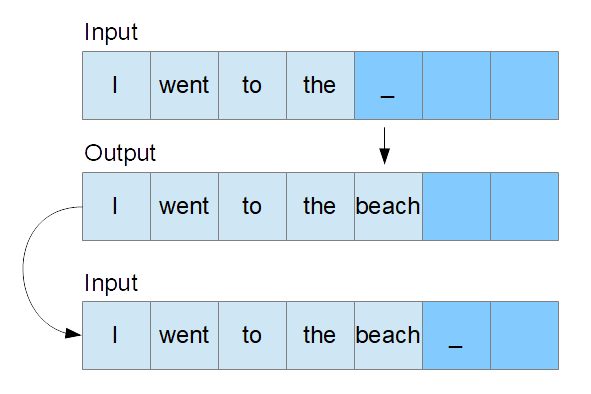
\includegraphics[height=5cm]{pics/autoregressives_modell.png}
\caption{Konzept eines autoregressiven Modells}
\label{fig:autoregressive}
\end{figure}
Das urspr\"ungliche \textbf{GPT}-Modell besteht aus 12 solcher Decoder-Bl\"ocke, die hintereinander durchgangen werden. Die folgenden Modelle bieten auch jeweils eine Version mit 12 Decodern, dies ist aber immer die kleinste Version. Die gr\"o{\ss}te Version von \textbf{GPT-2 } umschlie{\ss}t 48 Decoder-Schichten, w\"ahrend \textbf{GPT-3} bis 96 Schichten hat. Das momentan gr\"o{\ss}te GPT-Modell hat somit mit Decoder-Parametern und eigenen Parametern f\"ur Positional Encoding und Embedding 175 Milliarden Parameter, ein gro{\ss}er Schritt nach den 1,5 Milliarden von \textbf{GPT-2}.\\
 Es ist ein Meilenstein f\"ur teil\"uberwachtes und auch un\"uberwachtes Lernen: \textbf{GPT-3} kann Aufgaben teilweise im Ansatz l\"osen, ohne Beispiele gesehen zu haben oder auch f\"ur diese Aufgabe gelernt zu haben. Besser funktioniert aber die \textbf{Few-Shot}-Technik: Man zeigt dem Modell eine gewisse Anzahl (unterer zweistelliger Bereich oder weniger) an Beispielen der Aufgabe, die gel\"ost werden soll und fragt danach ab. Dies ist aufgrund der wenig vorhandenen gelabelten Datens\"atze ein gro{\ss}er Vorteil dieses Modells.\\

\textbf{Input und Output}\\
\textbf{GPT} arbeitet als Input mit sogenannten \textbf{Kontexten}: Dazu geh\"oren hier die Beschreibung der zu erf\"ullenden Aufgabe, eventuelle Beispiele und der \textbf{Prompt}, der dazu auffordert, die Aufgabe mit dem Prompt als Input zu l\"osen. Ein Beispiel f\"ur einen Kontext ist \cite{gpt3}:
\begin{verbatim} 
A "whatpu" is a small, furry animal native to Tanzania. 
An example of a sentence that uses the word whatpu is:
We were traveling in Africa and we saw these very cute whatpus.
To do a "farduddle" means to jump up and down really fast. 
An example of a sentence that uses the word farduddle is:
\end{verbatim} 
Diese Aufgaben und S\"atze sind von Menschen geschrieben als Input an das \textbf{GPT}-Modell gegeben worden. Die in Anf\"uhrungszeichen stehenden W\"orter sind frei erfunden, um zu zeigen, wie das Sprachmodell mit neuen W\"ortern umgeht. Der von \textbf{GPT} generierte Output ist:
\begin{verbatim} 
One day when I was playing tag with my little sister, she got  
really excited and she started doing these crazy farduddles.
\end{verbatim} 
Viel Feinabstimmung braucht \textbf{GPT-3} damit nicht mehr, was einer enormen Zeitersparnis entspricht. Die Vorg\"angermodelle sowie auch \textbf{GPT-3} f\"ur bessere Ergebnisse sollten jedoch mit einem \"uberwachten Trainingsschritt fein abgestimmt werden.\\

\textbf{Trainingsdaten}\\
Die genutzten Trainingsdaten sind ein wesentlicher Unterschied der Versionen: Das erste Modell wurde mit verschiedenen Datensets trainiert, die zusammen eine Gr\"o{\ss} von knapp \"uber 15GB erreichen, darunter die 1B Word Benchmark und PG-19. F\"ur \textbf{GPT-2} wurden ca. 40GB Daten genutzt, enthalten in dem Datensatz \textbf{WebText}, der f\"ur diese Aufgabe erstellt wurde. Die f\"ur \textbf{GPT-3} verwendeten Daten hingegen umfassen \"uber 500GB alleine mit dem genutzten Teil des \textbf{CommonCrawl} Datensatzes, der Texte aus dem Internet von 2016 bis 2019 enth\"alt und auf Duplikate \"uberpr\"uft wurde. Weiterhin wurden das eigene \textbf{WebText2} und die Datens\"atze \textbf{Books1}, \textbf{Books2} und das englischsprachige Wikipedia. Die Batchsize dieses Modells ist 0,5 Millionen. Das Modell \"ubertrifft damit an Gr\"o{\ss}e bei Weitem das, was bis zu seiner Ver\"offentlichung vorhanden war.\\
Wichtig zu beachten ist, dass diese Modelle aufgrund der Qualit\"at der generierten Texte, die gr\"o{\ss}tenteils nicht mehr von von Menschen geschriebenen zu unterscheiden sind, auch gewisse Risiken bergen \cite{gpt3}: Es ist deutlich einfacher, damit Fake News und Fehlinformationen zu generieren und zu verbreiten.


\subsection{BERT}
Wie auch \textbf{GPT} basiert \textbf{BERT} auf der Idee, einen Teil des \textbf{Transformers} zu gebrauchen, um ein Sprachmodell zu erstellen.\\

\textbf{Architektur}\\
Bei \textbf{BERT} wird im Unterschied zu \textbf{GPT} nicht der \textbf{Decoder}, sondern der \textbf{Encoder} genutzt: Es gibt zwei Versionen von \textbf{BERT}, die kleinere (\textbf{BERT Base}) besteht aus 12 Encoder-Schichten - genannt \textbf{Transformer-Bl\"ocke}, w\"ahrend \textbf{BERT Large} 24 Bl\"ocke (und damit 340 Millionen Parameter) umfasst \cite{bert}. Zur Zeit seiner Ver\"offentlichung stellte \textbf{BERT} f\"ur viele Aufgaben in NLP die state-of-the art Ergebnisse.\\
Schon am Namen dieses Sprachmodells kann man erkennen, das es nach dem Modell von \textbf{ELMo} kommen soll: Die von \textbf{GPT} nicht genutzte, aber in \textbf{ELMo} sehr erfolgreich angewandte Bidirektionalit\"at sollte wieder eingef\"uhrt werden. Dies hat den Hintergrund, dass in Sprache nicht nur die W\"orter wichtig f\"ur den Kontext eines bestimmten Wortes sind, die im Satz davor stehen - vielmehr ist die ganze Sequenz wichtig, um den ganzen Kontext zu erfassen. Ein reines Feed-Forward-Netz ist dazu nicht in der Lage. Die \textbf{Transformer}-Architektur bietet aufgrund der \textbf{Self-Attention}-Schichten eine gewisse M\"oglichkeit f\"ur bidirektionalen Kontext. Um dies auszunutzen, wird \textbf{BERT} mit verschiedenen Datens\"atzen und zu einem gewissen Grad randomisiert vortrainiert. Zu diesem Vortraining gibt es zwei Komponenten, die in einem Schritt ausgef\"uhrt werden. \textbf{BERT} erh\"alt dezu als Input zwei S\"atze. Das \textbf{Masked Language Model} wird mit jedem der beiden S\"atze trainiert, in denen zuf\"allig W\"orter maskiert werden, was effektiv einem L\"uckentext entspricht. \textbf{BERT} muss nun lernen, die in dem Satz fehlenden W\"orter einzusetzen. Die ausgegebenen Wortvektoren der maskierten W\"orter werden mit einer Output-Schicht mit dem Vokabular entsprechender Anzahl an Neuronen (hier 30000, das Vokabular von \textbf{WordPieces}) mit Softmax in eine Wahrscheinlichkeitsverteilung umgewandelt und mit einer one-hot codierten Version des tats\"achlichen Wortes abgeglichen. Auch m\"oglich ist, dass statt der Maskierung ein Wort durch ein nicht in den Satz passendes ersetzt wird und das Modell diesen Fehler korrigieren soll. Ebenso wird \textbf{Next Sentence Prediction} umgesetzt, bei der das Modell  ausgibt, ob die beiden als Input gegebenen S\"atze korrelieren. Der Output wird, wie bei \textbf{Transformern} \"ublich, parallel \"uber eine gesamte Eingabesequenz ausgegeben.\\
F\"ur die Feinabstimmung des Sprachmodells werden die Parameter der Output-Schicht durch einen aufgabenspezifischen Datensatz neu erlernt.\\

\textbf{Input und Output}\\
Als Input verarbeitet \textbf{BERT} Sequenzen, wobei hier spezielle Tokens genutzt werden. Das [MASK]-Token ersetzt maskierte W\"orter w\"ahrend des Vortrainings, um zu signalisieren, welche W\"orter untersucht werden m\"ussen. Diese Mechanik kann aber auch Probleme erzeugen, da das Token nur w\"ahrend des Vortrainings vorkommt: Bei Feinabstimmung und Test ist es nicht vorhanden, es kann daher nicht mit Sicherheit gesagt werden, wie \textbf{BERT} lernt, damit umzugehen \cite{xlnetex}.\\
Zu Beginn einer Sequenz wird das Token [CLS] gesetzt, das als Platzhalter f\"ur den Klassifikator fungiert. Der Klassifikator wird nach Verarbeitung durch \textbf{BERT} mit einem aus einer einzigen Schicht bestehenden Feed-Forward-Netz mit Softmax bestimmt. Soll mehr als ein Label ausgegeben werden muss hier die Anzahl an Output-Neuronen angepasst werden. F\"ur die anderen W\"orter der Sequenz werden die erstellten Wortvektoren ausgegeben, bei \textbf{BERT Base} haben diese 768 Dimensionen.\\
Das Token [SEP] wird gebraucht, um zwei zusammenh\"angende Sequenzen zu trennen, z.B. bei Frage/Antwort-Paaren. Hierbei wird dan an der Position des [CLS]-Tokens kein Klassifikator mehr ausgegeben, sondern die Wahrscheinlichkeit, das der Satz nach [SEP] auf den Satz vor dem Token folgt.\\
So kann \textbf{BERT} f\"ur die verschiedensten Aufgaben verwendet werden. Aber auch die reinen Word Embeddings k\"onnen ausgelesen und in einem eigenen erstellten Netz f\"ur weitere Aufgaben verwendet werden. Da jeder Decoder-Block des Modells einen eigenen Vektor f\"ur jedes Wort ausgeben kann, muss man im Einsatz dabei jedoch darauf achten, welche dieser Schichten die am besten Kontextualisierung des Wortes darstellt. In Tests der Entwickler erreichte hierbei eine Verkettung der letzten vier Schichten die besten Ergebnisse \cite{bert}.\\
Das Embedding der W\"orter in der Vorverarbeitung folgt einer \textbf{Byte Pair Codierung} auf Buchstabenebene.\\

\textbf{Trainingsdaten}\\
Zum Vortraining von \textbf{BERT} wurden die englischsprachigen \textit{Wikipedia} Artikel sowie BookCorpus mit insgesamt 13GB genutzt.


\subsection{RoBERTa}
Da \textbf{BERT} ein sehr vielversprechendes Modell war, wurde versucht, dieses zu optimieren, ohne die urspr\"ungliche Architektur zu \"andern. Ein besonderer Fokus lag dabei auf den [MASK]-Tokens, die in keinem anderen Sprachmodell verwendet werden \cite{roberta}.\\

\textbf{Architektur}\\
Die hier benutzte Architektur ist im Grunde die in \textbf{BERT} genutzte. Verschiedene Parameter wurden dabei ge\"andert, wie die h\"ochste verwendete Lernrate und den Epsilon-Paramater des Adam Optimizers.\\

\textbf{Input und Output}\\
Insgesamt wurde \textbf{RoBERTa} am deutlichsten \"uber den Input beim Vortraining ge\"andert. Trotz der besseren Ergebnisse bei \textbf{BERT} durch die parrallel zum \textbf{Masked Language Model} ausgewerteten \textbf{Next Sentence Prediction} werden bei \textbf{RoBERTa} diese Ergebnisse nicht best\"atigt. Bei der Implementation von \textbf{RoBERTa} wurde \textbf{NSP} entsprechend weggelassen.\\
Die Encodierung der Sequenzen in der Vorverarbeitung wurde ebenfalls ge\"andert: Es wird eine \textbf{Byte Pair Codierung} auf Byte-Ebene (entgegen Buchstabenebene bei \textbf{BERT}) genutzt. Dadurch werden die W\"orter unterteilt, das Vokabular umfasst 50000 solcher Wortteile. Durch diese Embeddings kommen bis zu 20 Millionen Parameter zu den \textbf{BERT}-Versionen hinzu.\\
Es werden ebenfalls l\"angere Batches mit einer Gr\"o{\ss}e von 8000 verwendet und die Trainingsdaten werden in l\"angere Sequenzen aufgeteilt. Der Einsatz der [MASK]-Tokens wird hier auch ein wenig abge\"andert: Statt die Tokens einmal f\"ur die Daten zu bestimmen - wenn auch zuf\"allig - werden sie bei \textbf{RoBERTa} dynamisch bestimmt. Dies hat den Vorteil, dass das Modell, wenn es einen Satz zum zweiten Mal sieht, dieser nur mit sehr geringer Wahrscheinlichkeit dieselbe Verteilung der Tokens hat. Dadurch kann das Modell den Kontext insgesamt besser erfassen.\\

\textbf{Trainingsdaten}\\
Da auch die Entwickler von \textbf{BERT} schon angermerkt hatten, dass ein gr\"o{\ss}erer Trainingsdatensatz f\"orderlich f\"ur die Performanz des Modells sein w\"urde, wurde dies hier umgesetzt. Zus\"atzlich zu den voher verwendeten 13GB an BookCorpus und Wikitext werden die Datens\"atze \textbf{CC-News}, \textbf{OpenWebText} (eine frei verf\"ugbare Version des in \textbf{GPT} genutzten Datensatzes) und \textbf{STORIES} eingesetzt, um insgesamt 160GB an Trainingsdaten zu erhalten, die das Modell dadurch insgesamt nicht so h\"aufig sieht. Damit ist das Modell deutlich gr\"o{\ss}er als das urspr\"ungliche \textbf{BERT}.


\subsection{XLNet}
\textbf{XLNet} basiert auf zwei Schl\"usselideen: Der Einsatz einer \textbf{RNN}-\"ahnlichen Struktur, um noch mehr Kontext zu erfassen, als mit dem ursp\"unglichen \textbf{Transformer}-Modell m\"oglich ist, und das Konzept von \textbf{BERT} so anzupassen, dass Maskierung im Training nicht mehr gebraucht wird, um eventuelle Fehler zu umgehen \cite{xlnetex}.

\subsubsection*{Transformer XL}
In diesem Sprachmodell wird eine Abwandlung der \textbf{Transformer} genutzt. Da diese Sequenzen parallel verarbeiten, gibt es eine obere Grenze and W\"ortern, die gleichzeitig verarbeitet werden k\"onnen, die darin resultiert, dass auch die Anzahl an W\"ortern, die als Kontext gelernt werden begrenzt ist. Diese Grenze ist aufgrund der heutigen Rechenm\"oglichkeiten recht hoch \cite{xlnetex}, aber sie existiert. Die Entwickler haben daher eine Technik erfunden, die die Funktionsweise eines \textbf{RNNs} nachbildet: Der Status des Netzes wird nach Verarbeitung einer Sequenz eingefroren und der folgenden Sequenz als Input mitgegeben. Dadurch k\"onnen auch sehr lange Sequenzen "`ganz"' verarbeitet werden. Dabei entsteht allerdings das Problem, das bei dem urspr\"unglichen \textbf{Transformer} durch \textbf{Positional Encoding} gel\"ost wurde: Das Modell kann einem Wort im Satz keine Position mehr zuordnen, da alles parallel verarbeitet wird. Dies wird im \textbf{Transformer XL} durch \textbf{relative positional embedding} umgangen. Durch dieses Embedding wird die relative Position eines Wortes zu einem anderen codiert, sodass die \textbf{Attention}-Werte f\"ur diese relative Relation korrekt bestimmt werden k\"onnen.

\textbf{Architektur}\\
Der Aufbau des Modelles gleicht dem von \textbf{BERT}, mit 12 Schichten und den gleich gew\"ahlten Hyperparametern sowie einer Sequenzl\"ange von 512 hat das Modell eine sehr \"ahnliche Gr\"o{\ss}e. Der Unterschied besteht hier nur in der Nutzung von \textbf{Transformer XL} statt der urspr\"unglichen Version. Diese lieferten bessere Ergebnisse, auch ohne Nutzung der im Folgenden erw\"ahnten Permutation.

\textbf{Input und Output}\\
Um die Maskierung zu umgehen, die bei \textbf{BERT} im Vortraining sehr wichtig ist, wird bei \textbf{XLNet} die Idee der \textbf{Permutationsmodellierung} eingef\"uhrt. Der dadurch entstehende Unterschied wird in Abbildung \ref{fig:xlnet} verdeutlicht.
\begin{figure}[!ht]
\centering
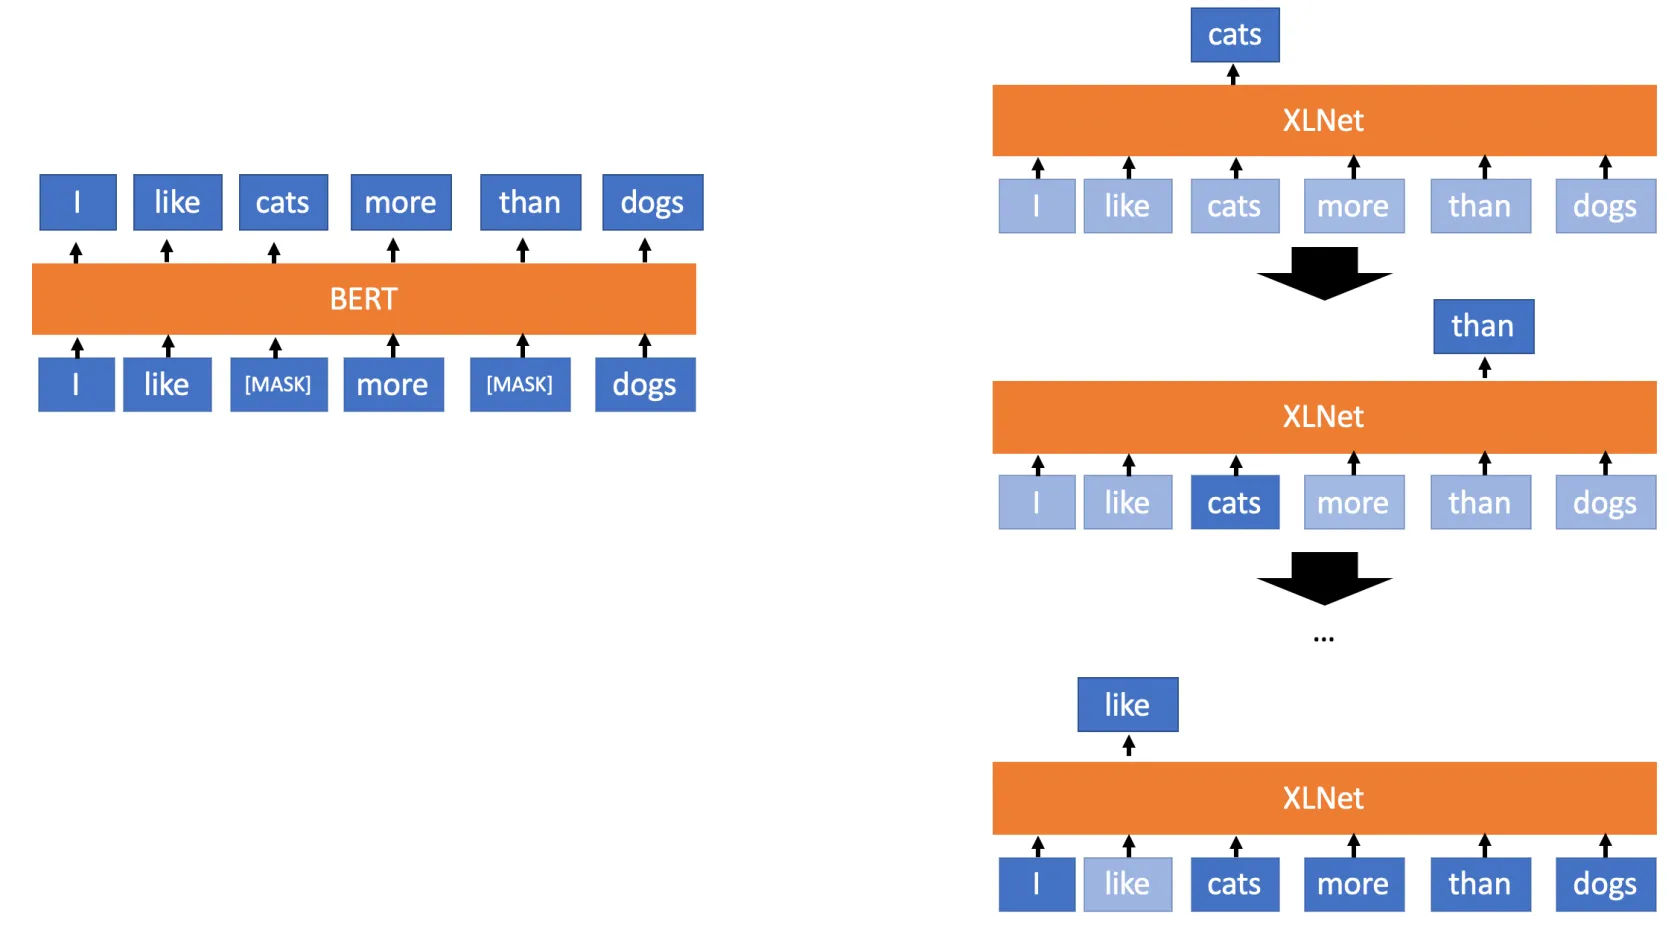
\includegraphics[height=5cm]{pics/xlnet_vs_bert.png}
\caption{Unterschied der Textgenerierung von BERT zu XLNet: Permutation \cite{xlnetex}}
\label{fig:xlnet}
\end{figure}
W\"ahrend mit \textbf{BERT} alle Wortvektoren inklusive dem im Input maskierten parallel ausgegeben werden, findet hier bei \textbf{XLNet} eine Permutation statt: Die Vektoren werden in einer zuf\"allig gew\"ahlten Reihenfolge ausgegeben. Dies gibt dem Modell auch wieder die M\"oglichkeit der Nutzung des Konzepts der Autoregressivit\"at, das bei fr\"uheren Modellen erfolgreich eingesetzt wurde. Zu der autoregressiven Eigenschaft kommt durch die Permutation eine Bidirektionalit\"at, da W\"orter zu beiden Seiten des n\"achsten im Input sein k\"onnen.\\

\textbf{Trainingsdaten}\\
Die bei \textbf{BERT} bew\"ahrten Trainingsdaten \textbf{BookCorpus} und der englischsprachige Teil von \textit{Wikipedia} werden auch hier eingesetzt. Zus\"atzlich werden \textbf{Giga5}, \textbf{ClueWeb} und \textbf{Common Crawl} in einer ges\"auberten Version benutzt, sodass insgesamt 126GB an Textdaten verwendet werden.


%%
%% Kapitel
%%
\chapter{Einsatz von Sprachmodellen}
Im Zuge dieser Arbeit wurden Versuche mit verschiedenen Sprachmodellen durchgef\"uhrt, die im Folgenden beschrieben werden.

\section{Versuchsaufbau}
Der Source Code f\"ur die Versuche ist in Python verfasst, da die Sprachmodelle alle eine \"ubersichtliche Schnittstelle zur Verwendung in Python bieten. Die erstellten Netze sind durch die Bibliotheken \textit{keras} \cite{keras} und \textit{Tensorflow} \cite{tensorflow} implementiert worden. \\
Der Code wurde zum Testen in \textbf{Jupyter Notebooks} auf Googles Plattform \textit{Google Colab} \cite{colab} ausgef\"uhrt, da mit dieser Plattform eine Laufzeitumgebung mit M\"oglichkeit zur Nutzung von einer GPU sowie - falls n\"otig - einer TPU zur Verf\"ugung steht. Die genaue Spezifikation der GPU kann dabei nicht ausgew\"ahlt werden, es sind \textit{Nvidia K80s, T4s, P4s} und \textit{P100s} verf\"ugbar \cite{colab_gpu}. Die genutzten Datens\"atze werden \"uber Links zu der Datenquelle (\textit{kaggle.com, github.com}) oder lokal eingebunden. F\"ur mehrere der Sprachmodelle waren dies nicht genug Ressourcen, deshalb wurden diese Experimente in einer docker-Umgebung auf einem GPU-Server ausgef\"uhrt, in der 16 Tesla V100-SXM3 zur Verf\"ugung standen. Die Batch Gr\"o{\ss}e wurde den jeweils verf\"ugbaren Ressourcen angepasst.\\
Als Vergleichswerte zwischen den Sprachmodellen wurden die Genauigkeiten bei der Auswertung der jeweiligen Datens\"atze sowie die \textbf{F1-score} hergenommen. Der \textbf{F1-Wert} berechnet sich wie in Gleichung 3.1 beschrieben, wobei \textit{tp} f\"ur \textit{true positives}, \textit{fp} f\"ur \textit{false positives} und \textit{tp} f\"ur \textit{true negatives} stehen \cite{f1}.
\begin{align}
   F1 {=} \frac{tp}{tp + \frac{1}{2} \dot (fp + fn)}
\end{align}
Die Zeit zum Ausf\"uhren wurde gemessen, gibt aber aufgrund der unterschiedlichen genutzten GPUs keine hohe Aussagekraft sondern blo{\ss} einen ungef\"ahren Richtwert bei Nutzung einer GPU.

\subsection{Verwendete Bibliotheken}
F\"ur die verschiedenen Sprachmodelle ist die Nutzung mehrer Bibliotheken f\"ur python n\"otig. Diese werden in dem jeweiligen Notebook eingebunden und teilweise zur Laufzeit installiert. Die wichtigsten dieser Bibliotheken sind im Folgenden aufgestellt:
\begin{itemize}
\item \textbf{Tensorflow}
\item \textbf{Fastai}
\item \textbf{Torch}
\item \textbf{gpt}
\item \textbf{simpletransformers} \cite{simpletransformers} f\"ur die Einbindung der transformerbasierten Sprachmodelle
\item \textbf{sklearn} f\"ur Auswertung der Ergebnisse
\item \textbf{nltk, pandas, string} und andere Standardbibliotheken f\"ur Textverarbeitung 
\end{itemize}
Die \textbf{SimpleTransformers} Bibliothek baut auf der Transformer-Bibliothek von \textbf{HuggingFace} auf und bietet einige Funktionen, um den Umgang mit Transformer-Modellen zu erleichtern. Die Effizienz dieser Bibliothek wurde in dieser Arbeit ebenfalls getestet.

\section{Die Daten}
F\"ur \textbf{Sentiment Analysis} werden ausschlie{\ss}lich Daten genutzt, die von der Plattform \textit{Twitter} genommen wurden. Diese Daten eignen sich sehr gut f\"ur diese Aufgabe, da die L\"ange der Textst\"ucke auf 280 Zeichen begrenzt ist \cite{twitter} und es eine gro{\ss}e Nutzerbasis und damit eine gro{\ss}e Vielfalt an formulierten Texten gibt. Hierbei werden die Tweets genommen, die nur Text und entsprechende Emojis enthalten und in Englisch verfasst sind. Die genutzten Datens\"atze sind gelabelt, um damit \textbf{Supervised Learning} zu betreiben, da die Feinabstimmung der Sprachmodelle so erfolgen muss.\\
Die Daten werden alle vorverarbeitet, um die Texte einheitlich und gut verarbeitbar zu machen. Hierzu werden f\"ur die Tweets folgende Schritte durchgangen:
\begin{itemize}
\item alle W\"orter in Kleinbuchstaben umwandeln
\item doppelte Buchstaben entfernen (aus "`helloooo"' wird z.B. "`hello"') 
\item Whitespaces an Anfang und Ende entfernen
\item Emojis entfernen
\end{itemize}
Die Daten f\"ur den Teil \textbf{Stance detection} haben unterschiedliche Urspr\"unge. Datens\"atze bestehen aus Artikeln, deren \"Uberschriften und den jeweiligen angesprochenen Stances, oder Tweets und der Haltung des Autors zu einem bestimmten, ebenfalls enthaltenen Thema. Auch diese Daten werden einer Datenreinigung unterzogen. Diese unterscheidet sich nur leicht von der f\"ur die \textbf{Sentiment Analysis} durchgef\"uhrte, da die Artikel im Allgemeinen keine sogenannten \textit{handles} oder Emojis enthalten. Diese Datens\"atze sind gelabelt, um einen sp\"ateren Test m\"oglich zu machen.\\
Wie bei sehr vielen Machine Learning Aufgaben h\"angen die Ergebnisse stark von der Qualit\"at der genutzten Daten ab. Es wurde demnach versucht, alle Datens\"atze so zu reinigen, dass die Performanz optimal wurde. Auf etwaige zus\"atzliche Schritte wird in der jeweiligen Beschreibung eingegangen.\\
Die Datens\"atze werden in Test- und Trainingsdaten aufgeteilt, wobei der Anteil der Testdaten 33\% des gesamten Datensatzes ist.

%subsections für die verschiedenen Datensätze 

\subsection{Apple Sentiment}
\label{sec:applesent}
Dieser Datensatz ist manuell gelabelt und wurde urspr\"unglich von \textit{crowdflower} \cite{crowdflower} zur Verf\"ugung gestellt. Die 1624 englischsprachigen Tweets wurden aufgrund von \textit{hashtags} gefiltert, die die Firma \textit{Apple} betreffen. Die hier verwendete Version \cite{apple_sent} ist soweit gefiltert, dass nur Tweets und Labels enthalten sind. Alle nicht relevanten Tweets wurden ebenfalls entfernt. Die Labels dieses Datensatzes sind -1 (negativ), 0 (neutral) und 1 (positiv). Der Datensatz ist dabei unbalanciert, mit 42\% an negativen, 49\% neutralen und 9\% positiven Tweets.\\
\lstset{language=Python}
\lstset{frame=lines}
\lstset{caption={S\"auberung des Datensatzes}}
\lstset{captionpos=b}
\lstset{label={lst:clean_140}}
\lstset{basicstyle=\footnotesize}
\begin{lstlisting}
df_train.tweet = df_train.tweet.str.lower()
df_test.tweet = df_test.tweet.str.lower()

# Delete URLs
df_train.text = df_train.text.apply(lambda x:re.sub(r'http\S+', '', x))
df_test.text = df_test.text.apply(lambda x:re.sub(r'http\S+', '', x))

#Tokenize, better for emojis, double characters and handle stripping than pure text
tokenizer = TweetTokenizer(strip_handles=True, reduce_len=True)
df_train.tweet = df_train.tweet.apply(lambda x: tokenizer.tokenize(x))
df_test.tweet = df_test.tweet.apply(lambda x: tokenizer.tokenize(x))

# Detokenize for better processing
df_train.tweet = df_train.tweet.apply(lambda x: ' '.join(x))
df_test.tweet = df_test.tweet.apply(lambda x: ' '.join(x))

df_train.tweet = df_train.tweet.map(lambda x : 
	x.translate(str.maketrans('', '', string.punctuation)))
df_test.tweet = df_test.tweet.map(lambda x : 
	x.translate(str.maketrans('', '', string.punctuation)))

df_train.tweet = df_train.tweet.str.replace("[0-9]", " ")
df_test.tweet = df_test.tweet.str.replace("[0-9]", " ")

df_train.tweet = df_train.tweet.str.strip(string.whitespace)
df_test.tweet = df_test.tweet.str.strip(string.whitespace)

# Recreate index that was shuffeled when splitting test and train
df_train = df_train.reset_index(drop=True)
df_test = df_test.reset_index(drop=True)
\end{lstlisting}
In diesem Datensatz sind keine Emojis enthalten, die entfernt werden m\"ussten. Die S\"auberung erfolgt wie in Listing \ref{lst:clean_140} dargestellt und das Ergebnis ist in folgender Tabelle dargestellt:

%Beispiele aus gesäubertem Datensatz
\begin{center}
\begin{tabular}{|c|c|}
\hline
tweet & sentiment\\ 
\hline\hline
the secret of life from steve jobs in    seconds& \\ some motivation from the late ceo of&0\\
\hline
it took just one month for the iphone plus& \\to become the king of phablets  is king  jobspring technews&1\\
\hline
imessage isnt working thanks&-1\\
\hline    
\end{tabular}
\end{center}


\subsection{US Airline Sentiment}
\label{sec:airlinesent}
Wie auch der Datensatz aus Teil \ref{sec:applesent} wurde der \textbf{US Airline Sentiment} durch Anwendung von Filtern von \textit{Twitter} bezogen \cite{airlines}. Der Datensatz besteht aus 14640 in Englisch verfassten Tweets mit manuell gelabelten Meinungen der Nutzer zu verschiedenen Fluggesellschaften. Die Einteilung der Sentiment-Werte ist hier als Label statt numerisch gegeben: Es gibt die Labels \textit{neutral, negative} und \textit{positive}. Zur Verarbeitung durch die Sprachmodelle wurden diese Labels jeweils numerisch codiert. Auch dieser Datensatz ist unbalanciert: 63\% sind negativ, 21\% neutral und 16\% positiv.\\
Da in den Texten noch Emojis vorhanden sind, werden diese durch den in Listing \ref{lst:clean_airline} gezeigten Code entfernt. Es wurden ebenfalls Versuche mit noch enthaltenen Emojis durchgef\"uhrt. Beispiele aus dem ges\"auberten Datensatz sind in der folgenden Tabelle gegeben.
%Code zur Säuberung
\lstset{language=Python}
\lstset{frame=lines}
\lstset{caption={Funktion zum Entfernen von Emojis}}
\lstset{captionpos=b}
\lstset{label={lst:clean_airline}}
\lstset{basicstyle=\footnotesize}
\begin{lstlisting}
def remove_emoji(string):
    emoji_pattern = re.compile("["
                           u"\U0001F600-\U0001F64F"  # emoticons
                           u"\U0001F300-\U0001F5FF"  # symbols & pictographs
                           u"\U0001F680-\U0001F6FF"  # transport & map symbols
                           u"\U0001F1E0-\U0001F1FF"  # flags (iOS)
                           u"\U00002702-\U000027B0"
                           u"\U000024C2-\U0001F251"
                           "]+", flags=re.UNICODE)
    return emoji_pattern.sub(r'', string)
\end{lstlisting}
%Beispiele aus gesäubertem Datensatz
\begin{center}
\begin{tabular}{|c|c|}
\hline
tweet & sentiment\\ 
\hline\hline
youre my early frontrunner for best airline  oscars&positive\\
\hline
what is going on with your bdl to dca flights yesterday&\\ and today   why is every single one getting delayed&negative\\
\hline
do they have to depart from washington  d  c&neutral\\
\hline    
\end{tabular}
\end{center}

\subsection{T4SA}
\label{sec:t4sa}
Der \textbf{T4SA} Datensatz \cite{t4sa} wurde von seinen Entwicklern zur \textbf{Cross-Media-Analyse} genutzt. Hierbei wurden zun\"achst die Texte der Tweets nach sentiment-Werten klassifiziert, um die ebenfalls in den Tweets enthaltenen Bilder zu labeln. Auch diese Tweets wurden gefiltert um sicherzustellen, dass alle Tweets Bilder enthalten, in Englisch verfasst und mindestens f\"unf W\"orter lang sind. In dieser Arbeit stehen die enthaltenen Bilder nicht zur Betrachtung, aber der zu Sentiment-Werten gelabelte Datensatz l\"asst sich gut verwenden.\\
Hier genutzt werden 1179957 der im Datensatz enthaltenen Tweets. Diese Teilmenge besteht nur aus mit Sentiment-Werten versehenen Tweets. Dabei sind 15\% negativ, 53\% neutral und 31\% positiv. Da die Daten auf mehrere Dateien verteilt sind, ist eine etwas aufwendigere Vorverarbeitung notwendig: Zus\"atzlich zu der in Listing \ref{lst:clean_140} und \ref{lst:clean_airline} aufgef\"uhrten Testverarbeitung werden die beiden Dateien in einen Dataframe zusammengefasst, indem die Tweet-ID jeweils als Schl\"usselwert genommen wird. Die Sentiment-Werte liegen in der Original-Datei als in drei Spalten (\textit{POS, NEG} und \textit{NEU}) aufgeteilte Wahrscheinlichkeitswerte vor. Der Spaltenname mit der h\"ochsten eingetragenen Wahrscheinlichkeit wird im Folgenden als das Label der Zeile genommen und in den Modellen entsprechend numerisch codiert. Beispiele aus dem final genutzten Dataframe sind in der folgenden Tabelle aufgef\"uhrt.
%Beispiele aus gesäubertem Datensatz
\begin{center}
\begin{tabular}{|c|c|}
\hline
tweet & sentiment\\ 
\hline\hline
inbound marketing content ideas part&NEU\\
\hline
i think this song is about phil im excited&POS\\
\hline
yo this the ugliest filter eveeer son  im weaaak&NEG\\
\hline    
\end{tabular}
\end{center}

\subsection{Fake News Challenge}
\label{sec:tfnc}
Dieser Datensatz besteht aus 49972 Artikeln, verschiedenen Aussagen, die \"uber den Text (oder einen anderen) getroffen wurden und der Beziehung zwischen den Aussagen und den Artikeln \cite{fnc}. Beziehungen werden in die Kategorien "`unrelated"', "`agree"', "`discuss"' und "`disagree"' eingeordnet. Diese Klassifizierung wurde f\"ur die Verarbeitung durch die Modelle numerisch codiert. Der Inhalt ist unbalanciert, 73\% der Trainingsdaten sind mit "`unrelated"', 18\% mit "`discuss"' und die restlichen 9\% mit "`disagree"' oder "`agree"' gelabelt. Da es sich hier um Artikel handelt, m\"ussen bei der Datenreinigung keine Emojis oder \textit{Twitter-Handles} beachtet werden. Die in unterschiedlichen Dateien vorliegenden Artikel werden den Aussagen zugeordnet und danach in Kleinbuchstaben umgewandelt. Zeichensetzung sowie Whitespaces an Anfang und Ende des Artikels werden entfernt. Gek\"urzte Beispiele aus dem Datensatz sind im Folgenden gelistet.
%Beispiele aus gesäubertem Datensatz
\begin{center}
\begin{tabular}{|c|c|c|}
\hline
Aussage & Artikel & Stance\\ 
\hline\hline
 mexico says students not& more graves have been discovered at  & discuss\\
 among dead in mass grave & the site where 43 students went missing &\\
\hline
isis beheads american & afghanistan veteran sam arnold uploaded this & unrelated\\
 photojournalist james wright & spinechilling  video of a us marine getting &\\
 foley threatens more to come & a direct headshot from a taliban sniper [...] &\\
\hline    
\end{tabular}
\end{center}

\subsection{SemEval}
\label{sec:semeval}
\textbf{SemEval} wurde urspr\"unglich f\"ur einen ausgeschriebenen Wettbewerb erstellt \cite{semeval}. In diesem Datensatz sind 2814 Tweets enthalten, die gegen unterschiedliche \textbf{Targets} auf ihre Haltung \"uberpr\"uft wurden. Die Haltung ist klassifiziert durch die Kategorien "`AGAINST"' (48\%), "`FAVOR"' (26\%) und "`NONE"' (26\%). Auch hier wurden die Kategorien numerisch codiert. Die S\"auberung l\"auft analof zu der S\"auberung der Tweets in den vorangegangenen Datens\"atzen. Die Themen dieses Wettbewerbs sind \textit{Hillary Clinton, Donald Trump, Atheismus, Feminismus, Klimawandel ist real} und \textit{das Recht auf Abtreibung}.

%Beispiele aus gesäubertem Datensatz
\begin{center}
\begin{tabular}{|c|c|c|}
\hline
Target & Tweet & Stance\\ 
\hline\hline
 hillary clinton & and  handovertheserver she wiped clean  30k deleted & AGAINST\\
  & emails  explains dereliction of duty  lies re benghazi  etc tcot semst  &\\
\hline
hillary clinton & hillary is our best choice if we truly want to & FAVOR\\
&  continue being a progressive nation  ohio semst &\\
\hline    
\end{tabular}
\end{center}

\section{Sentiment Analysis}
Im Folgenden werden die Experimente zu \textbf{Sentiment Analysis} im Detail beschrieben. Hierbei wird zun\"achst das verwendete Modell beschrieben und dann auf die spezifischen Aspekte wie Codierung der Labels und Ergebnisse zu den verschiedenen Datens\"atze eingegangen. 

\subsection{Ausgangsbasis}
Um einen Vergleich zu haben, wie performant und genau \textbf{Sentiment Analysis} mit Sprachmodellen ist, wurde zun\"achst ein Ansatz ausgewertet, der keinen Gebrauch von Deep Learning macht. Die Ver\"anderung der Genauigkeit im Vergleich zu diesem Ansatz gibt einen Anhaltspunkt, wie viel Sprachmodelle in Sentiment Analysis leisten k\"onnen.\\
Der jeweilige Datensatz wird mit pythons \textit{pandas} Bibliothek eingelesen, ges\"aubert und im Anschluss mit der Bibliothek \textit{TextBlob} ausgewertet. Diese Auswertung basiert auf manuell erstellten Dokumenten, in denen allen W\"ortern Sentiment-Werte zugeordnet wurden. \textit{TextBlob} werten diese Werte f\"ur einen gegebenen Text aus und gibt einen Wert zwischen -1 und 1 zur\"uck (negativ zu positiv). Um mit den Labels der Datents\"atze vergleichbar zu sein, wurden diese float-Werte zur jeweils n\"achsten ganzen Zahl gerundet. Da diese Auswertung sequentiell erfolgt, wurde keine GPU genutzt. Die Auswertung erfolgt durch den in Listing \ref{lst:code_direct} aufgezeigten Code. Um besser vergleichbar zu sein, wurde, wie in den anderen Modellen jeweils nur der Test-Dataframe ausgewertet.
%Code zu TextBlob
\lstset{language=Python}
\lstset{frame=lines}
\lstset{caption={Auswertung mit TextBlob}}
\lstset{captionpos=b}
\lstset{label={lst:code_direct}}
\lstset{basicstyle=\footnotesize}
\begin{lstlisting}
data.insert(2, "blobpolarity", 
	data.text.map(lambda x: int(round(TextBlob(x).sentiment.polarity)), 
	True)
\end{lstlisting}

\subsubsection*{Apple Sentiment}
Die Einstufungen m\"ussen bei diesem Datensatz nicht umgerechnet werden. Aufgrund der begrenzten Anzahl an Daten in dem Datensatz dauert die Berechnung der Sentiment-Werte unter einer Minute. Der Genauigkeitswert liegt bei 53,0\%.

\subsubsection*{US Airline Sentiment}
In diesem Datensatz werden die Labels in eine numerische Form gebracht, sodass die Werte analog zum letzten Experiment bei -1, 0 und 1 liegen. Auch bei diesem Datensatz dauert die Auswertung unter einer Minute. Es wird eine Genauigkeit von 25,7\% erreicht.

\subsubsection*{T4SA}
Wie in dem \textbf{US Airline Sentiment} Datensatz werden die Labels numerisch codiert. Die Auswertung dauert 3 Minuten und ergibt eine Genauigkeit von 66,1\%.

\subsubsection*{Auswertung}
Die Genauigkeitswerte schwanken stark, da kein Lernvorgang stattfindet und alle Datens\"atze nach dem gleichen Prinzip ausgewertet werden, obwohl sie an sich unterschiedliche Sprachaspekte enthalten. Die h\"aufigste Klassifizierung von TextBlob ist "`Neutral"', wodurch die \textbf{F1-Score} hier jeweils am h\"ochsten ist. Die Datens\"atze sind dabei nicht ganz ausgeglichen und in den Tests\"atzen \textbf{Apple Sentiment} und \textbf{T4SA} sind mehr neutral klassifizierte Tweets enthalten, was sich in der h\"oheren Genauigkeit niederschl\"agt.
\begin{center}
\begin{tabular}{|c||c|c|c|}
\hline
F1 score & Apple Sentiment & US Airline Sentiment & T4SA\\ 
\hline\hline
-1 & 0,156 & 0,098 & 0,185\\
\hline
0 & 0,675 & 0,349 & 0,758\\ 
\hline
1 & 0,286 & 0,283 & 0,543\\
\hline    
\end{tabular}
\end{center}

%ELMo
\subsection{ELMo}
Die verwendeten Datens\"atze werden zun\"achst ges\"aubert und in einen Dataframe eingelesen. Daraufhin wird das \textbf{ELMo-Modell} geladen und die Vektoren f\"ur die Eingabe bestimmt: Hierbei wird f\"ur eine Eingabesequenz ein einziger Vektor durch Mittelwertbildung bestimmt, um eine gute Weiterverarbeitung zu garantieren. Diese 1024-dimensionalen Vektoren werden abgespeichert, um immer auf sie zugreifen zu k\"onnen.\\
Da \textbf{ELMo} kein eigenes Modell zur Sentiment Analysis bietet, werden hier zwei verschiedene Ans\"atze erprobt:
\begin{itemize}
\item Logistic Regression
\item einschichtiges LSTM-Netz
\end{itemize}
Bei der \textbf{Logistischen Regression} wird eine Funktion gesucht, die die Beziehung zwischen den \textbf{ELMo}-Vektoren und den Labels des Datensatzes modelliert.\\
Das einschichtige LSTM-Netz wurde mithilfe von \textit{keras} implementiert, der Input ist der 1024-dimensionale Wortverktor. Dieser wird in eine LSTM-Schicht mit 512 Neuronen gegeben, um danach in einer \textbf{fully connected} Schicht weiterverarbeitet und zu einem drei Labels umfassenden Output gemappt, wie Listing \ref{lst:elmo_lstm_model} zeigt. Die Anzahl der zu trainierenden Epochen wurde anhand des \textbf{Validation Loss} bestimmt.
\lstset{language=Python}
\lstset{frame=lines}
\lstset{caption={Aufbau des LSTM-Netzes}}
\lstset{captionpos=b}
\lstset{label={lst:elmo_lstm_model}}
\lstset{basicstyle=\footnotesize}
\begin{lstlisting}
_________________________________________________________________
Layer (type)                 Output Shape              Param #   
=================================================================
lstm_1 (LSTM)                (None, 512)               3147776   
_________________________________________________________________
dense_1 (Dense)              (None, 3)                 1539      
_________________________________________________________________
activation_1 (Activation)    (None, 3)                 0         
=================================================================
\end{lstlisting}

\subsubsection*{Apple Sentiment}
Die Bestimmung der Wortvektoren dauert ca. 15 Sekunden, die Auswertung erfolgt in unter einer Sekunde. Mit der \textbf{Logistischen Regression} wird eine Genauigkeit von 83,8\% erreicht. Das LSTM-Netz wird in 20 Epochen trainiert und liefert eine Genauigkeit von 82,0\%.

\subsubsection*{US Airline Sentiment}
\textbf{ELMo} Wortvektoren sind nach 45 Sekunden berechnet, die Berechnung der \textbf{Logistischen Regression} dauert eine halbe Minute. Dadurch wird eine Genauigkeit von 81,0\% erreicht.  Aus dem wieder in 20 Epochen trainierten LSTM-Netz folgt eine Genauigkeit von 81,5\%.

\subsubsection*{T4SA}
Die L\"ange des Datensatzes wirkt sich in einer l\"angeren Berechnungszeit aus: Die Wortvektoren sind nach 40 Minuten bestimmt. Auch die Berechnung der \textbf{Logistischen Regression} dauert mit 4 Minuten etwas l\"anger und das in 20 Epochen trainierte LSTM-Modell braucht 30 Minuten. Die erreichten Genauigkeiten liegen bei 92,8\% bzw. 95,4\%.

\subsubsection*{Auswertung}
Die erreichten Genauigkeiten wie auch die \textbf{F1}-Werte weisen darauf hin, dass bei der Arbeit mit \textbf{ELMo}-Vektoren der Einsatz von \textbf{Logistischer Regression} bei kleineren Datens\"atzen ausreichend ist, um ein Modell zu bestimmen, ein LSTM-Netz gibt kaum Verbesserungen. Da der \textbf{T4SA}-Datensatz gr\"o{\ss} ist, kann das LSTM-Netz l\"anger trainiert werden und erreicht dementsprechend bessere Ergebnisse als die \textbf{Logistische Regresseion}. Die in diesem Experiment errechneten Genauigkeiten sind weit von state-of-the-art-Ergebnissen entfernt.\\
Man kann erkennen, dass die ersten beiden Datens\"atze zu negativen Sentiments unbalanciert sind, mit einem l\"angeren Datensatz scheint dies aber ausgeglichen - hier ist das dritte Label h\"aufig genug vorhanden.
\textbf{Logistische Regression}
\begin{center}
\begin{tabular}{|c||c|c|c|}
\hline
F1 score & Apple Sentiment & US Airline Sentiment & T4SA\\ 
\hline\hline
-1 & 0,857 & 0,884 & 0,855\\
\hline
0 & 0,862 & 0,632 & 0,950\\ 
\hline
1 & 0,5 & 0,730 & 0,925\\
\hline    
\end{tabular}
\end{center}

\textbf{LSTM-Netz}
\begin{center}
\begin{tabular}{|c||c|c|c|c|}
\hline
F1 score & Apple Sentiment & US Airline Sentiment & T4SA\\ 
\hline\hline
-1 & 0,843 & 0,887 & 0,904\\
\hline
0 & 0,845 & 0,642 & 0,969\\ 
\hline
1 & 0,419 & 0,728 & 0,953\\
\hline    
\end{tabular}
\end{center}

%ULMFit
\subsection{ULMFit}
Dieses Modell wurde nach dem Beispiel in \cite{ulm_model} implementiert. Zun\"achst werden die Textdaten importiert und gereinigt. Dabei wird f\"ur alle Datens\"atze au{\ss}er \textbf{Sentiment140} eine \textbf{one-hot-Codierung} ausgef\"uhrt, da mit dem Modell Multi-Klassen Klassifizierung sonst nicht m\"oglich ist. Dies resultiert in drei neuen Spalten in den Dataframes (negativ, neutral und positiv), die jeweils bin\"ar codiert sind.\\

\lstset{language=Python}
\lstset{frame=lines}
\lstset{caption={Laden des ULMFit Modells}}
\lstset{captionpos=b}
\lstset{label={lst:load_ulm_train}}
\lstset{basicstyle=\footnotesize}
\begin{lstlisting}
learn = language_model_learner(data_lm, drop_mult=0.7, 
		arch = AWD_LSTM, pretrained = True)
\end{lstlisting}

Daraufhin wird das geladene \textbf{ULMFit} Sprachmodell mit den Tweet-Texten der Trainingsdaten initialisiert und verschiedene Lernraten mittels eines Lernratenfinders ausprobiert. Wie der Grafik \ref{fig:lr_ulmfit} zu entnehmen ist, ist die gew\"ahlte Lernrate 0,01.
\begin{figure}[!ht]
\centering
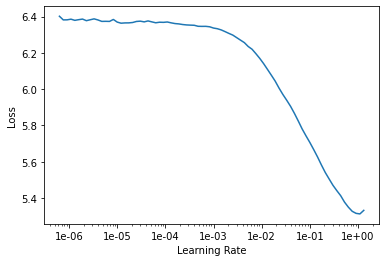
\includegraphics[height=5cm]{pics/lr_finder_ulmfit.png}
\caption{Lernratenfinder}
\label{fig:lr_ulmfit}
\end{figure}
Der n\"achste Schritt besteht aus dem \textbf{unfreezing} der Gewichte und dem Trainieren des Sprachmodells mit den Textdaten. Dazu wird die Anzahl der Epochen an den jeweiligen Datensatz angepasst. Es wird eine Anzahl gew\"ahlt, die der Gr\"o{\ss}e des Datensatzes angemessen ist und nach dem \textbf{Validation Loss} entschieden, wann gestoppt wird: Die maximale Anzahl der Epochen ist erreicht, sobald das \textbf{Validation Loss} h\"oher wird um \textbf{Overfitting} zu vermeiden. Die daraus errechneten Gewichte werden f\"ur die sp\"atere Verwendung abgespeichert.\\
Danach wird der \textbf{Classifier} trainiert. Dieser erh\"alt als Input die Textdaten und die drei Spalten f\"ur die Labels und wird nach den Metriken \textit{Genauigkeit, precision} und \textit{recall} trainiert. Mit \textbf{gradual unfreezing} werden zun\"achst nur die letzten zwei Schichten des Modells angepasst und im n\"achsten Schritt noch einmal alle Schichten trainiert. Dieser Vorgang kann dem Listing \ref{lst:code_clas_ulm_train} entnommen werden.
\lstset{language=Python}
\lstset{frame=lines}
\lstset{caption={Gradual Unfreezing zum Trainieren des Classifiers}}
\lstset{captionpos=b}
\lstset{label={lst:code_clas_ulm_train}}
\lstset{basicstyle=\footnotesize}
\begin{lstlisting}
learn.freeze_to(-2)
learn.fit_one_cycle(2, slice(1e-2/(2.6**4),1e-2), moms=(0.8,0.7), wd=0.1)

learn.unfreeze()
learn.fit_one_cycle(2, slice(1e-3/(2.6**4),1e-3), moms=(0.8,0.7), wd=0.1)
\end{lstlisting}

\subsubsection*{Apple Sentiment}
Auch bei diesem Modell dauert das Trainieren des Modells in 20 Epochen und des Classifiers mit dem Datensatz unter einer Minute. Mit einer GPU kann hier schon ein gewisser Grad an Parallelisierung stattfinden.  Erreichte Genauigkeiten liegen bei 82,4\%. 


\subsubsection*{US Airline Sentiment}
Durch die \textbf{one-hot-Codierung} des Datensatzes f\"allt die anderweitige numerische Codierung der Labels weg. Die ermittelte Anzahl an Epochen, die das Sprachmodell trainiert wird, liegt bei zehn. Damit dauert das Training des Sprachmodells 50 Sekunden. Die Feinabstimmung des Classifiers dauert eine weitere Minute, es werden Genauigkeiten bis 88,5\% erreicht.

\subsubsection*{T4SA}
Die Vorverarbeitung verl\"auft analog zu der des \textbf{US Airline Sentiment} Datensatzes. Das Sprachmodell wird aufgrund der Menge der Daten 10 Epochen trainiert, die Trainingsdauer liegt damit bei ca 90 Minuten. Die Feinabstimmung des Classifiers dauert weitere 90 Minuten und die Genauigkeit liegt am Ende bei 97,5\%. Dieser Datensatz w\"urde von l\"angerem Training noch einen gro{\ss}en Nutzen ziehen: Nach den vergangegen Epochen war noch ein starker sinkender Trend im \textbf{Validation Loss}  zu erkennen. Dies kann mit der Gr\"o{\ss}e des Datensatzes zusammenh\"angen, da kaum M\"oglichkeiten zum \textbf{Overfitting} bestehen.

\subsubsection*{Auswertung}
Hier kann sehr gut beobachtet werden, wie sich die Gr\"o{\ss}e des Datensatzes auf die Ergebnisse auswirkt: Die steigende Genauigkeit und \textbf{F1-Scores} zeigen, dass das Modell daran insgesamt besser trainieren kann. Die Gefahr des \textbf{Overfitting} ist ebenfalls sehr gering und das Modell k\"onnte insgesamt l\"anger als hier angegeben trainiert werden.
\begin{center}
\begin{tabular}{|c||c|c|c|}
\hline
F1 score & Apple Sentiment & US Airline Sentiment & T4SA\\ 
\hline\hline
-1 & 0,743 & 0,896 & 0,957\\
\hline
0 & 0,783 & 0,670 & 0,986\\ 
\hline
1 & 0,25 & 0,756 &  0,981\\
\hline    
\end{tabular}
\end{center}

%RoBERTa
\subsection{RoBERTa}
F\"ur dieses Sprachmodell m\"ussen die Eingabedaten leicht angepasst werden: Die Labels werden in die Zahlen 0, 1 und 2 codiert, damit von dem Modell verarbeitet werden k\"onnen. F\"ur die in Text gegebenen Label wird dies mit einem \textit{dictionary} gel\"ost:
\lstset{language=Python}
\lstset{frame=lines}
\lstset{caption={Umkodieren der sentiment-Label}}
\lstset{captionpos=b}
\lstset{label={lst:dict_conv_sentiment}}
\lstset{basicstyle=\footnotesize}
\begin{lstlisting}
thisdict =	{
  "negative": 0,
  "neutral": 1,
  "positive": 2
}
df_train.sentiment = df_train.sentiment.apply(lambda x: thisdict[x])
df_test.sentiment = df_test.sentiment.apply(lambda x: thisdict[x])
\end{lstlisting}
Daraufhin wird das vortrainierte Modell von \textit{pytorch} geladen und auf Multi-Label-Erkennung konfiguriert.
\lstset{language=Python}
\lstset{frame=lines}
\lstset{caption={Laden und Konfigurieren des RoBERTa-Modells}}
\lstset{captionpos=b}
\lstset{label={lst:load_config_roberta}}
\lstset{basicstyle=\footnotesize}
\begin{lstlisting}
config = RobertaConfig.from_pretrained('roberta-base')
# Set number of output labels
config.num_labels = 3
\end{lstlisting}
Die Eingabetexte werden danach in \textbf{RoBERTa}-Tokens und weiterhin \textbf{CUDA}-Vektoren umgewandelt, um von der Parallelisierung durch GPUs Gebrauch zu machen. Hierbei gibt es Probleme mit dem Zero-Padding: Da das Modell die speziellen [CLS] und [SEP]-Tokens braucht, kann dies nicht einfach durchgef\"uhrt werden, was dazu f\"uhrt, dass die Batchg\"o{\ss}e nicht angepasst werden kann. \\
Das Modell wird im n\"achsten Schritt \"uber 10 Epochen mit einer Lernrate von $1^{-5}$ und dem \textbf{Adam-Optimizer} trainiert. Andere Lernraten wurden ausprobiert, gaben aber schlechtere Ergebnisse.\\
Eine alternative Version wurde mithilfe der \textbf{SimpleTransformers} Bibliothek implementiert. Diese hat den Vorteil, dass sie einfach zu nutzen und \"ubersichtlich ist, wie aus Listing \ref{lst:simple_roberta} hervorgeht.
\lstset{language=Python}
\lstset{frame=lines}
\lstset{caption={RoBERTa mit SimpleTransformers}}
\lstset{captionpos=b}
\lstset{label={lst:simple_roberta}}
\lstset{basicstyle=\footnotesize}
\begin{lstlisting}
from simpletransformers.classification import ClassificationModel

model = ClassificationModel('roberta', 'roberta-base', num_labels=3, args={
    'learning_rate':3e-5,
    'num_train_epochs': 10,
    'reprocess_input_data': True,
    'overwrite_output_dir': True,
    'process_count': 10,
    'train_batch_size': 4,
    'eval_batch_size': 4,
    'max_seq_length': 512,
    'n_gpu' : 4,
    'fp16': False
})

model.train_model(df_train)
\end{lstlisting}

\subsubsection*{Apple Sentiment}
Das Training \"uber zehn Epochen mit diesem Datensatz dauert eine halbe Stunde. Weniger Epochen f\"uhren dazu, dass der Classifier nur zwischen zwei Klassen unterscheiden kann und die dritte au{\ss}er Acht l\"asst, mit mehr Epochen steigt die Gefahr des \textbf{Overfitting}. Die erreichte Genauigkeit liegt bei 78,6\%, da die dritte Klasse nur selten erkannt wird.\\
Mit dem \textbf{SimpleTransformer} Modell dauert das Training mit zehn Epochen 15 Minuten und ergibt eine Genauigkeit von 88,7\%. Auch hier wird die dritte Klasse erst nach einigen Epochen Training erkannt. Weiteres Training f\"uhrt zu \textbf{Overfitting}

\subsubsection*{US Airline Sentiment}
Ohne \textbf{SimpleTransformers} wurde die Bearbeitung abgebrochen, da es so ineffizient ist, dass in 12 Stunden keine Epoche berechnet werden kann.
Die Bearbeitungzeit mit der \textbf{SimpleTransformers} Implementation lag bei 15 Epochen und 90 Minuten mit 16 GPUs, der Genauigkeitswert liegt damit bei 85,0\%.

\subsubsection*{T4SA}
Da selbst unter Einsatz des GPU-Servers eine Epoche \"uber neun Stunden zur Ausf\"uhrung braucht, kann dieser Datensatz im Rahmen der Arbeit nicht mit der eigenen Implementierung untersucht werden.
Mit \textbf{SimpleTransformers} dauert die Berechnung einer Epoche drei Stunden, liefert aber da schon eine Genauigkeit von 98,2\%.

\subsubsection*{Auswertung}
Das \textbf{RoBERTa}-Modell kann mit Multi-Klassen Umgebungen und unbalancierten Datens\"atzem nicht gut umgehen. Dies kann man besonders gut an den \textbf{F1}-Werten f\"ur das positive Label sehen: Um ein besseres Ergebnis zu erreichen muss mit vielen Daten lange trainiert werden. Die Implementierung an sich ist sehr ineffizient und kann daher mit gro{\ss}en Datens\"atzen nicht gut tainiert werden.
\begin{center}
\begin{tabular}{|c||c|c|c|}
\hline
F1 score & Apple Sentiment & US Airline Sentiment & T4SA\\ 
\hline\hline
-1 & 0,801 & - & -\\
\hline
0 & 0,826 & - & -\\ 
\hline
1 & 0,3 & - & -\\
\hline    
\end{tabular}
\end{center}
Auch bei \textbf{SimpleTransformers} kann man die Unbalanciertheit der Daten gut erkennen, mit langen Datens\"atzen ist dies ausgeglichen.
\begin{center}
\begin{tabular}{|c||c|c|c|}
\hline
F1 score & Apple Sentiment & US Airline Sentiment & T4SA\\ 
\hline\hline
-1 & 0,908 & 0,913 & 0,964\\
\hline
0 & 0,896 & 0,688 & 0,987\\ 
\hline
1 & 0,714 & 0,796 &  0,981\\
\hline    
\end{tabular}
\end{center}

%XLNet
\subsection{XLNet}
Wie auch bei dem \textbf{RoBERTa}-Modell werden hier die Labels so codiert, dass sie mit Indizes vergleichbar sind. Die f\"ur die Verarbeitung durch \textbf{XLNet} n\"otigen Tokens [SEP] und [CLS] werden an jeden Tweet angehangen und der Text wird mit einem XLNetTokenizer zu Tokens umgewandelt. Dies ergibt folgende Struktur f\"ur die Tweets:
\lstset{language=Python}
\lstset{frame=lines}
\lstset{caption={Tweet nach Tokenization}}
\lstset{captionpos=b}
\lstset{label={lst:tokenized_tweet}}
\lstset{basicstyle=\footnotesize}
\begin{lstlisting}
 ['_we',  '_need', '_more',   '_products',  '_like',  '_companies',  '_like',  '_need',  '_to',  '_embrace',  '_the',  '_customization',  '_of',  '_quality',  '_themes',  '[',  's',  'ep',  ']',  '_[',  'cl',  's',  ']']
\end{lstlisting}
Diese Tokens werden mit dem in Listing \ref{lst:tokenizer_ids} aufef\"uhrten Code in ids umgewandelt und daraufhin auf eine einheitliche L\"ange gebracht.
\lstset{language=Python}
\lstset{frame=lines}
\lstset{caption={Umwandlung in Ids}}
\lstset{captionpos=b}
\lstset{label={lst:tokenizer_ids}}
\lstset{basicstyle=\footnotesize}
\begin{lstlisting}
ids_train = [tokenizer.convert_tokens_to_ids(x) for x in tokenized_text_train]
input_ids_train2 = pad_sequences(ids_train,maxlen=MAX_LEN,dtype="long",
			truncating="post",padding="post")
\end{lstlisting}
Im n\"achsten Schritt werden die entstandenen IDs in Torch Tensoren gewandelt, um sie mit einem DataLoader verarbeiten zu k\"onnen.\\
Das vortrainierte \textbf{XLNet} wird geladen und auf die Anzahl der Labels (drei) konfiguriert. Mit dem \textbf{Adam-Optimizer} und einer Lernrate von $1^{-5}$ wird das Modell mit dem jeweiligen Datensatz trainiert. Andere Lernraten geben schlechtere Ergebnisse. Die Anzahl der zu lernenden Epochen wurde dem jeweiligen Datensatz angepasst.\\
Da es sich um ein transformerbasiertes Modell handelt, wurde eine Alternative zum oben beschriebenen Vorgehen mittel \textbf{SimpleTransformers} implementiert. Diese unterscheidet sich nur geringf\"ugig von dem in Listing \ref{lst:simple_roberta} aufgef\"uhrten Code, hier wird statt des \textbf{RoBERTa}-Modells \textbf{XLNet} geladen und trainiert.

\subsubsection*{Apple Sentiment}
Die Berechnung und Auswertung mit 40 Epochen Training dauert 20 Minuten und liefert eine Genauigkeit von 77,9\%. Bei wenigen Epochen wird auch hier das positive Label nicht mit einbezogen. Mehr Epochen f\"uhren bei dem kleinen Datensatz zu \textbf{Overfitting}.
Auf dem GPU-Server dauert das Training in f\"unf Epochen bei dem \textbf{SimpleTransformers}-Modell neun Minuten und erreicht eine bessere Genauigkeit als Training mit zehn Epochen. Der maximale Wert liegt hier bei 86,1\%.

\subsubsection*{US Airline Sentiment}
Das Training dauert bei ebenfalls 40 Epochen ca. 40 Minuten, die dabei erreichte Genauigkeit betr\"agt 66,2\%.
Der beste Genauigkeitswert des \textbf{SimpleTransformers} Modells wurde mit f\"unf Epochen Training in 35 Minuten erreicht (gg\"u. 15 Epochen). Er liegt bei 84,3\%.

\subsubsection*{T4SA}
Da selbst unter Einsatz des GPU-Servers eine Epoche \"uber neun Stunden zur Ausf\"uhrung braucht, kann dieser Datensatz im Rahmen der Arbeit nicht mit der eigenen Implementierung untersucht werden.
Die Implementation mit \textbf{SimpleTransformers} dauert unter Nutzung der 16 GPUs f\"unf Stunden f\"ur eine Epoche, liefert aber hier schon eine Genauigkeit von 98,0\%. Die Auswertung dauerte sechs Stunden.

\subsubsection*{Auswertung}
Auch hier ist zu beobachten, dass die Multi-Klassen Klassifizierung erst nach mindestens 10 Epochen funktioniert. Wieder empfiehlt es sich, bei den gr\"o{\ss}eren Datens\"atzen l\"anger zu lernen, bei den kleinen kann aufgrund von \textbf{Overfitting} nicht viel ge\"andert werden. Dies ist f\"ur beide Implementierungen der Fall, wie auch schon bei \textbf{RoBERTa}. Wieder ist die \textbf{SimpleTransformer}-Implementierung effizienter und liefert bessere Ergebnisse.
\begin{center}
\begin{tabular}{|c||c|c|c|}
\hline
F1 score & Apple Sentiment & US Airline Sentiment & T4SA\\ 
\hline\hline
-1 & 0,763 & 0,809 & -\\
\hline
0 & 0,836 & 0,283 & -\\ 
\hline
1 & 0,447 & 0,320 & -\\
\hline    
\end{tabular}
\end{center}
\textbf{SimpleTransformers}
\begin{center}
\begin{tabular}{|c||c|c|c|}
\hline
F1 score & Apple Sentiment & US Airline Sentiment & T4SA\\ 
\hline\hline
-1 & 0,877 & 0,906 & 0,961\\
\hline
0 & 0,879 & 0,668 & 0,986\\ 
\hline
1 & 0,632 & 0,794 & 0,980\\
\hline    
\end{tabular}
\end{center}

%GPT
\subsection{GPT}
Das von \textit{OpenAI} direkt bereitgestellte \textbf{GPT}-Modell wurde ebenfalls getestet, ergab aber auch nach intensivem Training keine brauchbaren Ergebnisse. Die dazu aufgestellte These ist, dass die Daten im Gegensatz zu dem Trainingsdatensatz beim Vortraining zu wenig und die Texte insgesamt zu kurz sind. Die jeweilige Ausgabe ergab teilweise eine sinnvolle Fortsetzung des voranstehenden Tweets, die tats\"achlichen Label wurden demnach nicht gelernt, wie in Listing \ref{lst:gpt_results} zu sehen ist. Es ist m\"oglich, dass mit sehr langem Training hier Ergebnisse erzielt werden k\"onnen, dies ist im Rahmen dieser Arbeit aber nicht durchf\"uhrbar.
\lstset{language=Python}
\lstset{frame=lines}
\lstset{caption={Ergebnisse des GPT-Modells}}
\lstset{captionpos=b}
\lstset{label={lst:gpt_results}}
\lstset{basicstyle=\footnotesize}
\begin{lstlisting}
Model prompt >>> // x bonus airmiles right now  airmilesshops ||
====================== SAMPLE 1 =========================
 noon 
======================================================
Model prompt >>> // since when did stop replacing iphone units due to defect  just because i have some scratches on my phone doesnt mean i dropped it ||
====================== SAMPLE 1 =========================
nooooooooooooooooo
======================================================
Model prompt >>> // i had to get my logic board completely replaced if its 
under warranty theyll do it for free  make sure to back up b ||
====================== SAMPLE 1 =========================
  
======================================================
Model prompt >>> // thanks for pushing me into yosemite it has been the worst
 so slow sand clunky  cantgoback misssnowleopard whathappened ||
====================== SAMPLE 1 =========================
 || cm
======================================================
\end{lstlisting}

\section{Stance Detection}
In den folgenden Unterkapiteln wird auf die Experimente zu \textbf{Stance Detection} eingegangen.

%ULMFit
\subsection{ULMFit}
Entsprechend dem Modell, dass f\"ur \textbf{Sentiment Analysis} genutzt wurde, wurde hier mit den Textdaten ein Sprachmodell antrainiert und anschlie{\ss}end der Classifier mit den Labels trainiert. Die Eingangsdaten wurden zur Verarbeitung der Klassen one-hot-codiert. Das vortrainitert fastai-Sprachmodell konnte ohne Probleme mit den zwei Textinputs umgehen.

\subsubsection*{FNC}
Nach insgesamt 210 Minuten Training \"uber 20 Epochen f\"ur das Sprachmodell und zehn f\"ur den Classifier liegt die Genauigkeit bei 94,5\%.

\subsubsection*{SemEval}
Aufgrund der kleinen Anzahl an Daten kann dieses Modell nicht gut trainiert werden. Das Training des Sprachmodells wie auch des Classifiers dauert unter einer Minute, nach acht Epochen sieht man durch steigendes \textbf{Validation Loss} (Abbildung \ref{fig:rising_validation}) hier schon einen Ansatz von \textbf{Overfitting}. Die erreichte Genauigkeit liegt bei 40,1\%.
\begin{figure}[!ht]
\centering
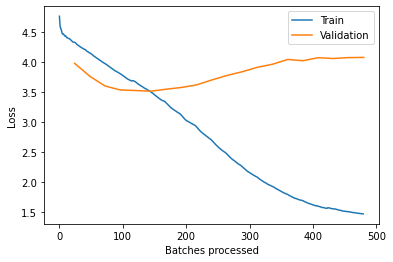
\includegraphics[height=5cm]{pics/rising_validation_loss.png}
\caption{Steigendes Validation Loss}
\label{fig:rising_validation}
\end{figure}

\subsubsection*{Auswertung}
Die bei dem kleineren Datensatz (\textbf{SemEval}) erreichte Genauigkeit liegt unter der, die erreicht werden kann, wenn nur in eine Kategorie eingeordnet wird. Dies weist darauf hin, dass der Datensatz zu klein ist, um ihn in diesem Modell zu verwenden.\\
 Da der zweite Datensatz mit hoher Wahrscheinlichkeit nicht richtig ausgewertet werden kann, kann dar\"uber keine Aussage getroffen werden. Getestet wurde, ob zwischen den Trainings- und Testdatens\"atzen Dopplungen vorliegen. Dies war nicht der Fall, aber da verschiedene Stances mehrmals in beiden Datens\"atzen vorkommen, ist zu vermuten, dass das Ergebnis verf\"alscht ist. Es liegt aber weit \"uber den durch reines "`unrelated"' Kategorisieren erreichbaren 73\%. Da kein eigener Testdatensatz vorhanden ist, kann dies jedoch nicht \"uberpr\"uft werden. Der Genauigkeitswert steigt jedoch immer weiter mit fortlaufendem Training, daher wird angenommen, das \textbf{Overfitting} stattfindet, dass durch die Testdaten nicht aufgedeckt werden kann.
\begin{center}
\begin{tabular}{|c||c|c|}
\hline
F1 score & FNC & SemEval\\ 
\hline\hline
0 & 0,987 & 0,680\\
\hline
1 & 0,809 & 0,462\\ 
\hline
2 & 0,939 & 0,483\\
\hline
3 & 0,594 & -\\
\hline    
\end{tabular}
\end{center}

%RoBERTa
\subsection{RoBERTa}
Die Daten m\"ussen f\"ur das mit \textbf{SimpleTransformers} implementierte Training in einem Dataframe vorliegen, dass die Spalten "`text\_a"', "`text\_b"' und "`labels" hat. Entsprechend wurden die Daten umformatiert. Die Anzahl der Labels wurde entsprechend dem Datensatz angepasst. Mit einer Lernrate von $3^{-5}$ wurde das Modell f\"ur eine dem Datensatz angepassten Anzahl an Epochen trainiert.

\subsubsection*{FNC}
Das Trainieren in zehn Epochen mit 16 GPUs dauert 180 Minuten, die dabei erreichte Genauigkeit ist 99,2\%. Wie auch schon bei \textbf{ULMFit} angemerkt wurde, ist dieses Ergebnis mit hoher Wahrscheinlichkeit jedoch verf\"alscht.

\subsubsection*{SemEval}
Dieses Experiment wurde auf dem GPU-Server unter Einsatz von 16 GPUs ausgef\"uhrt. f\"unf Epochen brauchen dabei 15, zehn Epochen 19 und 15 Epochen 28 Minuten. Die erreichte Genauigkeit ist mit 62,6\% bei zehn Epochen maximal.

\subsubsection*{Auswertung}
Die erreichte Genauigkeit ist weit von einem Idealwert entfernt, gegen\"uber dem \textbf{ULMFit} Modell ist sie aber schon gen\"ugend hoch um zu sagen, dass dieses Modell besser lernt. Es ist wahrscheinlich, dass nicht genug Beispiele in dem Datensatz existieren, er ist zu klein.
\begin{center}
\begin{tabular}{|c||c|c|}
\hline
F1 score & FNC & SemEval\\ 
\hline\hline
0 & 0,999 & 0,678\\
\hline
1 & 0,965 & 0,560\\ 
\hline
2 & 0,983 & 0,586\\
\hline
3 & 0,932 & -\\
\hline    
\end{tabular}
\end{center}

%XLNet
\subsection{XLNet}
Beide Datens\"atze werden in die von \textbf{SimpleTransformers} ben\"otigte Form gebracht und ausgewertet. Die Konfiguration des \textbf{XLNet}-Modells ist analog zu der in \textbf{Sentiment Analysis} vorgestellten Variante, die Anzahl der Labels und Epochen wird entsprechend angepasst.\\
Es wurde eine weitere Version analog zu der in \textbf{Sentiment Analysis} besprochenen implementiert, in der die Textspalten codiert und in Tokens umgewandelt wurden. Hierzu wurden die zu analysierenden Texte nach dem [SEP]-Token an die Aussage bzw. das Target angehangen, das weitere Vorgehen ist identisch.

\subsubsection*{FNC}
Die eigene Implementation ist ineffizient und versucht, mehr Speicher auf einer Grafikkarte zu alloziieren, als vorhanden ist, daher konnte dieser Versuch nicht durchgef\"uhrt werden.
Bei Nutzung von \textbf{SimpleTransformers} dauert das Training von 10 Epochen vier Stunden, der Genauigkeitswert liegt bei 99,4\%.

\subsubsection*{SemEval}
Das nicht mit \textbf{SimpleTransformers} implementierte Modell wurde in zehn Minuten f\"ur 20 Epochen trainiert, kann aber nicht zwischen den eigentlichen Labels unterscheiden. Die Genauigkeit von 51,8\% ist davon abzuleiten, dass die Daten stark unbalanciert sind.\\
Das andere Modell erreichte nach 15 Epochen Training (32 Minuten mit 16 GPUs) eine Genauigkeit von 57,4\%.

\subsubsection*{Auswertung}
Das Modell ist in der Performanz schlechter als \textbf{RoBERTa}. Wieder kann man an den Werten auch die Qualit\"at und L\"ange der jeweiligen Datens\"atze erkennen.
\begin{center}
\begin{tabular}{|c||c|c|}
\hline
F1 score & FNC & SemEval\\ 
\hline\hline
0 & 0,999 & 0,649\\
\hline
1 & 0,976 & 0,525\\ 
\hline
2 & 0,986 & 0,487\\
\hline
3 & 0,966 & -\\
\hline    
\end{tabular}
\end{center}
Ohne \textbf{SimpleTransformers}
\begin{center}
\begin{tabular}{|c||c|c|}
\hline
F1 score & FNC & SemEval\\ 
\hline\hline
0 & - & 0,682\\
\hline
1 & - & 0\\ 
\hline
2 & - & 0\\
\hline
3 & - & -\\
\hline    
\end{tabular}
\end{center}

%%
%% Kapitel
%%
\chapter{Auswertung}
Im Folgenden werden die Ergebnisse aus den Experimenten des lezten Kapitels besprochen und m\"ogliche Verbesserungen angesprochen.

\section{Ergebnisse}
Bei \textbf{Sentiment Analysis} werden durch die Sprachmodelle schnell bessere Ergebnisse erreicht als ohne. Besonders die nicht-transformerbasierten Modelle sind zeitlich bei der Ausf\"uhrung sehr gut, die Genauigkeitswerte sind mit \"uber 80\% durchaus wettbewerbsf\"ahig (s. Abbildung \ref{fig:acc_sentiment}). Besonders \textbf{ULMFit} scheint gut geeignet f\"ur diese Aufgabe, da auch die Verarbeitungszeit hier, nicht wie bei den Transformer-Modellen, dem Datensatz angemessen ist. Ist ein gro{\ss}er Datensatz vorhanden, kann auch entsprechend gut trainiert werden. Die transformerbasierten Modelle scheinen deutlich resistenter gegen \textbf{Overfitting} auch bei kleinen Datens\"atzen zu sein, brauchen aber langes Training, um wirklich hohe Genauigkeiten zu erreichen. Das Problem scheint hierbei haupts\"achlich bei der Multi-Klassen Klassifizierung zu liegen, da diese Modelle l\"anger brauchen, um \"uber zwei Klassen hinaus zu klassifizieren. Die deutlich l\"angere Auf\"uhrungszeit stammt aus der h\"oheren Komplexit\"at der Transformer-Modelle.\\
\begin{figure}[!ht]
\centering
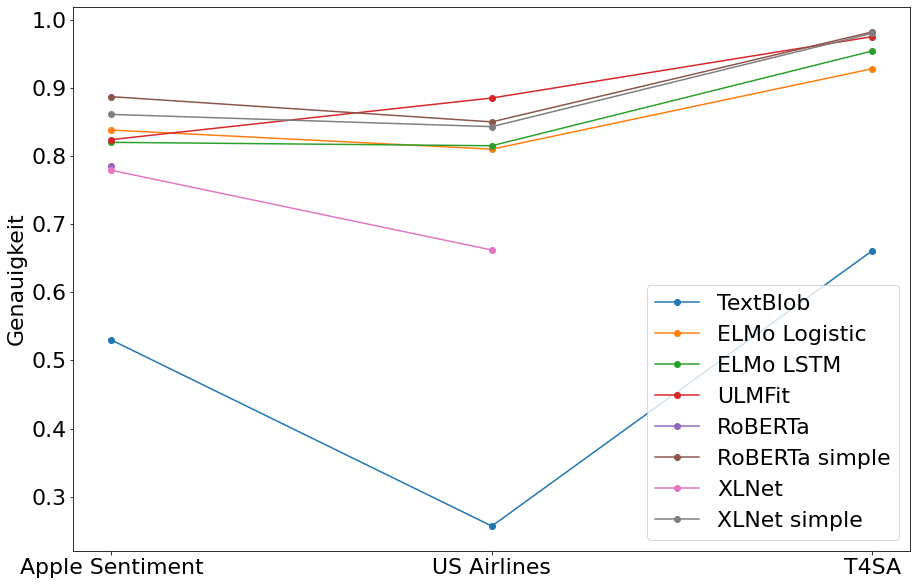
\includegraphics[height=8cm]{pics/accuracies_sentiment.png}
\caption{Genauigkeiten bei Sentiment Analysis}
\label{fig:acc_sentiment}
\end{figure}
Zur \textbf{Stance detection} scheinen LSTM-Modelle wie \textbf{ULMFit} weniger gut geeignet, hier werden die besten Ergebnisse durch Einsatz des \textbf{RoBERTa}-Modells mit \textbf{SimpleTransformers} erzielt, wie aus Abbildung \ref{fig:acc_stance} hervorgeht.
\begin{figure}[!ht]
\centering
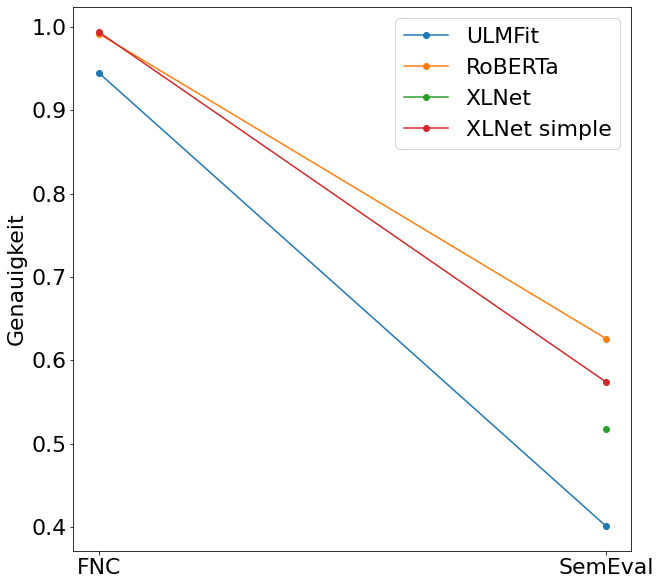
\includegraphics[height=8cm]{pics/accuracies_stance.png}
\caption{Genauigkeiten bei Stance Detection}
\label{fig:acc_stance}
\end{figure}
Aus den Graphen kann gefolgert werden, dass die mittels \textbf{SimpleTransformers} abgestimmten Modelle sehr effizient sind. Die Bibliothek ist offensichtlich gut anzuwenden und bringt sehr gute Ergebnisse. \\
Wie schon erw\"ahnt hat die Qualit\"at der und die Quantit\"at in den Datens\"atzen eine hohe Auswirkung auf das Ergebnis, dennoch kann gesagt werden, dass, wenn richtig konfiguriert, die urspr\"ungliche Transformer-Architektur der der XL-Transformer \"uberlegen ist.

\section{Ausblick}
In nachfolgenden Arbeiten kann die Trainingszeit und die Anzahl der getesteten Datensa\"atze erh\"oht werden, da die meisten Modelle von mehr Trainingszeit profitieren k\"onnen. Weiterhin k\"onnen auch bei der Textverarbeitung angebracht werden: Hierbei kann \textbf{Stemming} angewendet werden. Dadurch werden die W\"orter in ihre Grundform umgewandelt mit vorausgehenden oder nachfolgenden Silben als separate Tokens. Aus dem Wort "`playing"' werden so z.B. die zwei Tokens <play> und <ing>. Diese Art der \textbf{Tokenization} ist f\"ur den Einsatz mit Sprachmodellen am besten geeignet, da auch in diesen nicht alle Vokabeln einer Sprache enthalten sein k\"onnen - das w\"are schlicht ein zu gro{\ss}es Vokabular. Durch \textbf{Stemming} wird gew\"ahrleistet, dass die meisten W\"orter, sowie die jeweilige Pr\"afix und Suffix je einem Vektor zugeordnet werden k\"onnen (sollten keine Rechtschreibfehler enthalten sein).\\
Da \textbf{NLP} ein sehr weit verbreitetes Thema ist, werden auch in den n\"achsten Jahren immer weitere Sprachmodelle ver\"offentlicht werden, die in den unterschiedlichen Aufgabenstellungen St\"arken oder auch Schw\"achen haben werden und entsprechend getestet werden sollten.

\end{onehalfspace}

%% Abbildungsverzeichnis
\listoffigures

\begin{thebibliography}{}
%% Zitieren Sie diesen ersten Eintrag mit \cite{bib_1}
\bibitem{ulm} Howard, J., Ruder, S., Universal Language Model Fine-tuning for Text Classification. 2018,  arXiv:1801.06146 
\bibitem{attention} Vaswani, A. et al., Attention Is All You Need. 2017,  arXiv:1706.03762v5 
\bibitem{transformerxl} Dai, Z., Yang, Z., Yang,Y., Carbonell, J., Le, Q., Salakhutdinov, R., Transformer-XL: Attentive Language Models
Beyond a Fixed-Length Context. 2019,  arXiv:1901.02860v3 
\bibitem{elmo} Peters, M.,  Neumann, M.,  Iyyer, M., Gardner, M.,  Clark, C. , Lee, K., Zettlemoyer, L.,  Deep contextualized word representations. 2018, arXiv:1802.05365v2
\bibitem{elmoex} Mihail, E., Deep Contextualized Word Representations with ELMo. 2018, https://www.mihaileric.com/posts/deep-contextualized-word-representations-elmo/
\bibitem{bert} Devlin, J., Chang, M., Lee K. , Toutanova, K., BERT: Pre-training of Deep Bidirectional Transformers forLanguage Understanding. 2019, arXiv:1810.04805v2
\bibitem{roberta} Liu, Y., Ott, M., Goyal, N., Du, J., Joshi, M., Chen, D., Levy, O., Lewis, M., Zettlemoyer, L., Stoyanov, V., RoBERTa: A Robustly Optimized BERT Pretraining Approach. 2019, arXiv:1907.11692
\bibitem{gpt} Radford,  A.,  Narasimhan,  K.,  Salimans,  T.,  and  Sutskever,  I., Improving language understanding by generative pre-training. 2018, https://openai.com/blog/language-unsupervised/
\bibitem{gpt2} Radford, A., Wu, J., Child, R., Luan, D., Amodei, D., Sutskever, I., Language Models are Unsupervised Multitask Learners. 2018, https://openai.com/blog/better-language-models/
\bibitem{gpt3} Brown, T., Mann, B., Ryder, N., Subbiah, M., Kaplan, J., Dhariwal, P., Neelakantan, A., Shyam, P., Sastry, G., Askell, A., Agarwal, S., Herbert-Voss, A., Krueger, G., Henighan, T., Child, R., Ramesh, A., Ziegler, D., Wu, J., Winter, C., Hesse, C., Chen, M., Sigler, E., Litwin, M., Gray, S., Chess, B., Clark, J., Berner, C., McCandlish, S., Radford, A., Sutskever, I., Amodei, D., Language Models are Few-Shot Learners. 2020,  arXiv:2005.14165 
\bibitem{xlnet} Yang, Z., Dai, Z., Yang, Y., Carbonell, J., Salakhutdinov, R., Le, Q., XLNet: Generalized Autoregressive Pretraining
for Language Understanding. 2019, arXiv:1906.08237v2
\bibitem{xlnetex} Kurita, K., XLNet Explained. 2019,  https://mlexplained.com/2019/06/30/paper-dissected-xlnet-generalized-autoregressive-pretraining-for-language-understanding-explained/ 
\bibitem{sentiment140} Go, A., Bhayani, R., Huang, L., Twitter Sentiment Classification using Distant Supervision. 2009
\bibitem{twitter} So twitterst du. https://help.twitter.com/de/using-twitter/how-to-tweet
\bibitem{sentiment140} http://help.sentiment140.com/for-students
\bibitem{keras} https://keras.io/
\bibitem{tensorflow} https://www.tensorflow.org/
\bibitem{colab} https://colab.research.google.com/notebooks/intro.ipynb
\end{thebibliography}


\end{document}
